
%% bare_jrnl.tex
%% V1.4b
%% 2015/08/26
%% by Michael Shell
%% see http://www.michaelshell.org/
%% for current contact information.
%%
%% This is a skeleton file demonstrating the use of IEEEtran.cls
%% (requires IEEEtran.cls version 1.8b or later) with an IEEE
%% journal paper.
%%
%% Support sites:
%% http://www.michaelshell.org/tex/ieeetran/
%% http://www.ctan.org/pkg/ieeetran
%% and
%% http://www.ieee.org/

%%*************************************************************************
%% Legal Notice:
%% This code is offered as-is without any warranty either expressed or
%% implied; without even the implied warranty of MERCHANTABILITY or
%% FITNESS FOR A PARTICULAR PURPOSE! 
%% User assumes all risk.
%% In no event shall the IEEE or any contributor to this code be liable for
%% any damages or losses, including, but not limited to, incidental,
%% consequential, or any other damages, resulting from the use or misuse
%% of any information contained here.
%%
%% All comments are the opinions of their respective authors and are not
%% necessarily endorsed by the IEEE.
%%
%% This work is distributed under the LaTeX Project Public License (LPPL)
%% ( http://www.latex-project.org/ ) version 1.3, and may be freely used,
%% distributed and modified. A copy of the LPPL, version 1.3, is included
%% in the base LaTeX documentation of all distributions of LaTeX released
%% 2003/12/01 or later.
%% Retain all contribution notices and credits.
%% ** Modified files should be clearly indicated as such, including  **
%% ** renaming them and changing author support contact information. **
%%*************************************************************************


% *** Authors should verify (and, if needed, correct) their LaTeX system  ***
% *** with the testflow diagnostic prior to trusting their LaTeX platform ***
% *** with production work. The IEEE's font choices and paper sizes can   ***
% *** trigger bugs that do not appear when using other class files.       ***                          ***
% The testflow support page is at:
% http://www.michaelshell.org/tex/testflow/



\documentclass[journal]{IEEEtran}
%
% If IEEEtran.cls has not been installed into the LaTeX system files,
% manually specify the path to it like:
% \documentclass[journal]{../sty/IEEEtran}





% Some very useful LaTeX packages include:
% (uncomment the ones you want to load)


% *** MISC UTILITY PACKAGES ***
%
%\usepackage{ifpdf}
% Heiko Oberdiek's ifpdf.sty is very useful if you need conditional
% compilation based on whether the output is pdf or dvi.
% usage:
% \ifpdf
%   % pdf code
% \else
%   % dvi code
% \fi
% The latest version of ifpdf.sty can be obtained from:
% http://www.ctan.org/pkg/ifpdf
% Also, note that IEEEtran.cls V1.7 and later provides a builtin
% \ifCLASSINFOpdf conditional that works the same way.
% When switching from latex to pdflatex and vice-versa, the compiler may
% have to be run twice to clear warning/error messages.






% *** CITATION PACKAGES ***
%
%\usepackage{cite}
% cite.sty was written by Donald Arseneau
% V1.6 and later of IEEEtran pre-defines the format of the cite.sty package
% \cite{} output to follow that of the IEEE. Loading the cite package will
% result in citation numbers being automatically sorted and properly
% "compressed/ranged". e.g., [1], [9], [2], [7], [5], [6] without using
% cite.sty will become [1], [2], [5]--[7], [9] using cite.sty. cite.sty's
% \cite will automatically add leading space, if needed. Use cite.sty's
% noadjust option (cite.sty V3.8 and later) if you want to turn this off
% such as if a citation ever needs to be enclosed in parenthesis.
% cite.sty is already installed on most LaTeX systems. Be sure and use
% version 5.0 (2009-03-20) and later if using hyperref.sty.
% The latest version can be obtained at:
% http://www.ctan.org/pkg/cite
% The documentation is contained in the cite.sty file itself.






% *** GRAPHICS RELATED PACKAGES ***
%
\ifCLASSINFOpdf
   \usepackage[pdftex]{graphicx}
   \usepackage{subfigure} 
  % declare the path(s) where your graphic files are
  % \graphicspath{{../pdf/}{../jpeg/}}
  % and their extensions so you won't have to specify these with
  % every instance of \includegraphics
  % \DeclareGraphicsExtensions{.pdf,.jpeg,.png}
\else
  % or other class option (dvipsone, dvipdf, if not using dvips). graphicx
  % will default to the driver specified in the system graphics.cfg if no
  % driver is specified.
  % \usepackage[dvips]{graphicx}
  % declare the path(s) where your graphic files are
  % \graphicspath{{../eps/}}
  % and their extensions so you won't have to specify these with
  % every instance of \includegraphics
  % \DeclareGraphicsExtensions{.eps}
\fi
% graphicx was written by David Carlisle and Sebastian Rahtz. It is
% required if you want graphics, photos, etc. graphicx.sty is already
% installed on most LaTeX systems. The latest version and documentation
% can be obtained at: 
% http://www.ctan.org/pkg/graphicx
% Another good source of documentation is "Using Imported Graphics in
% LaTeX2e" by Keith Reckdahl which can be found at:
% http://www.ctan.org/pkg/epslatex
%
% latex, and pdflatex in dvi mode, support graphics in encapsulated
% postscript (.eps) format. pdflatex in pdf mode supports graphics
% in .pdf, .jpeg, .png and .mps (metapost) formats. Users should ensure
% that all non-photo figures use a vector format (.eps, .pdf, .mps) and
% not a bitmapped formats (.jpeg, .png). The IEEE frowns on bitmapped formats
% which can result in "jaggedy"/blurry rendering of lines and letters as
% well as large increases in file sizes.
%
% You can find documentation about the pdfTeX application at:
% http://www.tug.org/applications/pdftex





% *** MATH PACKAGES ***
%
%\usepackage{amsmath}
% A popular package from the American Mathematical Society that provides
% many useful and powerful commands for dealing with mathematics.
%
% Note that the amsmath package sets \interdisplaylinepenalty to 10000
% thus preventing page breaks from occurring within multiline equations. Use:
%\interdisplaylinepenalty=2500
% after loading amsmath to restore such page breaks as IEEEtran.cls normally
% does. amsmath.sty is already installed on most LaTeX systems. The latest
% version and documentation can be obtained at:
% http://www.ctan.org/pkg/amsmath





% *** SPECIALIZED LIST PACKAGES ***
%
%\usepackage{algorithmic}
% algorithmic.sty was written by Peter Williams and Rogerio Brito.
% This package provides an algorithmic environment fo describing algorithms.
% You can use the algorithmic environment in-text or within a figure
% environment to provide for a floating algorithm. Do NOT use the algorithm
% floating environment provided by algorithm.sty (by the same authors) or
% algorithm2e.sty (by Christophe Fiorio) as the IEEE does not use dedicated
% algorithm float types and packages that provide these will not provide
% correct IEEE style captions. The latest version and documentation of
% algorithmic.sty can be obtained at:
% http://www.ctan.org/pkg/algorithms
% Also of interest may be the (relatively newer and more customizable)
% algorithmicx.sty package by Szasz Janos:
% http://www.ctan.org/pkg/algorithmicx




% *** ALIGNMENT PACKAGES ***
%
%\usepackage{array}
% Frank Mittelbach's and David Carlisle's array.sty patches and improves
% the standard LaTeX2e array and tabular environments to provide better
% appearance and additional user controls. As the default LaTeX2e table
% generation code is lacking to the point of almost being broken with
% respect to the quality of the end results, all users are strongly
% advised to use an enhanced (at the very least that provided by array.sty)
% set of table tools. array.sty is already installed on most systems. The
% latest version and documentation can be obtained at:
% http://www.ctan.org/pkg/array


% IEEEtran contains the IEEEeqnarray family of commands that can be used to
% generate multiline equations as well as matrices, tables, etc., of high
% quality.




% *** SUBFIGURE PACKAGES ***
%\ifCLASSOPTIONcompsoc
%  \usepackage[caption=false,font=normalsize,labelfont=sf,textfont=sf]{subfig}
%\else
%  \usepackage[caption=false,font=footnotesize]{subfig}
%\fi
% subfig.sty, written by Steven Douglas Cochran, is the modern replacement
% for subfigure.sty, the latter of which is no longer maintained and is
% incompatible with some LaTeX packages including fixltx2e. However,
% subfig.sty requires and automatically loads Axel Sommerfeldt's caption.sty
% which will override IEEEtran.cls' handling of captions and this will result
% in non-IEEE style figure/table captions. To prevent this problem, be sure
% and invoke subfig.sty's "caption=false" package option (available since
% subfig.sty version 1.3, 2005/06/28) as this is will preserve IEEEtran.cls
% handling of captions.
% Note that the Computer Society format requires a larger sans serif font
% than the serif footnote size font used in traditional IEEE formatting
% and thus the need to invoke different subfig.sty package options depending
% on whether compsoc mode has been enabled.
%
% The latest version and documentation of subfig.sty can be obtained at:
% http://www.ctan.org/pkg/subfig




% *** FLOAT PACKAGES ***
%
%\usepackage{fixltx2e}
% fixltx2e, the successor to the earlier fix2col.sty, was written by
% Frank Mittelbach and David Carlisle. This package corrects a few problems
% in the LaTeX2e kernel, the most notable of which is that in current
% LaTeX2e releases, the ordering of single and double column floats is not
% guaranteed to be preserved. Thus, an unpatched LaTeX2e can allow a
% single column figure to be placed prior to an earlier double column
% figure.
% Be aware that LaTeX2e kernels dated 2015 and later have fixltx2e.sty's
% corrections already built into the system in which case a warning will
% be issued if an attempt is made to load fixltx2e.sty as it is no longer
% needed.
% The latest version and documentation can be found at:
% http://www.ctan.org/pkg/fixltx2e


%\usepackage{stfloats}
% stfloats.sty was written by Sigitas Tolusis. This package gives LaTeX2e
% the ability to do double column floats at the bottom of the page as well
% as the top. (e.g., "\begin{figure*}[!b]" is not normally possible in
% LaTeX2e). It also provides a command:
%\fnbelowfloat
% to enable the placement of footnotes below bottom floats (the standard
% LaTeX2e kernel puts them above bottom floats). This is an invasive package
% which rewrites many portions of the LaTeX2e float routines. It may not work
% with other packages that modify the LaTeX2e float routines. The latest
% version and documentation can be obtained at:
% http://www.ctan.org/pkg/stfloats
% Do not use the stfloats baselinefloat ability as the IEEE does not allow
% \baselineskip to stretch. Authors submitting work to the IEEE should note
% that the IEEE rarely uses double column equations and that authors should try
% to avoid such use. Do not be tempted to use the cuted.sty or midfloat.sty
% packages (also by Sigitas Tolusis) as the IEEE does not format its papers in
% such ways.
% Do not attempt to use stfloats with fixltx2e as they are incompatible.
% Instead, use Morten Hogholm'a dblfloatfix which combines the features
% of both fixltx2e and stfloats:
%
% \usepackage{dblfloatfix}
% The latest version can be found at:
% http://www.ctan.org/pkg/dblfloatfix




%\ifCLASSOPTIONcaptionsoff
%  \usepackage[nomarkers]{endfloat}
% \let\MYoriglatexcaption\caption
% \renewcommand{\caption}[2][\relax]{\MYoriglatexcaption[#2]{#2}}
%\fi
% endfloat.sty was written by James Darrell McCauley, Jeff Goldberg and 
% Axel Sommerfeldt. This package may be useful when used in conjunction with 
% IEEEtran.cls'  captionsoff option. Some IEEE journals/societies require that
% submissions have lists of figures/tables at the end of the paper and that
% figures/tables without any captions are placed on a page by themselves at
% the end of the document. If needed, the draftcls IEEEtran class option or
% \CLASSINPUTbaselinestretch interface can be used to increase the line
% spacing as well. Be sure and use the nomarkers option of endfloat to
% prevent endfloat from "marking" where the figures would have been placed
% in the text. The two hack lines of code above are a slight modification of
% that suggested by in the endfloat docs (section 8.4.1) to ensure that
% the full captions always appear in the list of figures/tables - even if
% the user used the short optional argument of \caption[]{}.
% IEEE papers do not typically make use of \caption[]'s optional argument,
% so this should not be an issue. A similar trick can be used to disable
% captions of packages such as subfig.sty that lack options to turn off
% the subcaptions:
% For subfig.sty:
% \let\MYorigsubfloat\subfloat
% \renewcommand{\subfloat}[2][\relax]{\MYorigsubfloat[]{#2}}
% However, the above trick will not work if both optional arguments of
% the \subfloat command are used. Furthermore, there needs to be a
% description of each subfigure *somewhere* and endfloat does not add
% subfigure captions to its list of figures. Thus, the best approach is to
% avoid the use of subfigure captions (many IEEE journals avoid them anyway)
% and instead reference/explain all the subfigures within the main caption.
% The latest version of endfloat.sty and its documentation can obtained at:
% http://www.ctan.org/pkg/endfloat
%
% The IEEEtran \ifCLASSOPTIONcaptionsoff conditional can also be used
% later in the document, say, to conditionally put the References on a 
% page by themselves.




% *** PDF, URL AND HYPERLINK PACKAGES ***
%
%\usepackage{url}
% url.sty was written by Donald Arseneau. It provides better support for
% handling and breaking URLs. url.sty is already installed on most LaTeX
% systems. The latest version and documentation can be obtained at:
% http://www.ctan.org/pkg/url
% Basically, \url{my_url_here}.




% *** Do not adjust lengths that control margins, column widths, etc. ***
% *** Do not use packages that alter fonts (such as pslatex).         ***
% There should be no need to do such things with IEEEtran.cls V1.6 and later.
% (Unless specifically asked to do so by the journal or conference you plan
% to submit to, of course. )


% correct bad hyphenation here
\hyphenation{op-tical net-works semi-conduc-tor}
\usepackage[utf8]{inputenc}
\usepackage[spanish]{babel}

\begin{document}
%
% paper title
% Titles are generally capitalized except for words such as a, an, and, as,
% at, but, by, for, in, nor, of, on, or, the, to and up, which are usually
% not capitalized unless they are the first or last word of the title.
% Linebreaks \\ can be used within to get better formatting as desired.
% Do not put math or special symbols in the title.
\title{Tarjeta SmartHouse para una habitación}
%
%
% author names and IEEE memberships
% note positions of commas and nonbreaking spaces ( ~ ) LaTeX will not break
% a structure at a ~ so this keeps an author's name from being broken across
% two lines.
% use \thanks{} to gain access to the first footnote area
% a separate \thanks must be used for each paragraph as LaTeX2e's \thanks
% was not built to handle multiple paragraphs
%

\author{John~Barahona,
        Cesar~Tejada,
        y~Cesar~Alvarez% <-this % stops a space
%\thanks{M. Shell was with the Department
%of Electrical and Computer Engineering, Georgia Institute of Technology, Atlanta,
%GA, 30332 USA e-mail: (see http://www.michaelshell.org/contact.html).}% <-this % stops a space
%\thanks{J. Doe and J. Doe are with Anonymous University.}% <-this % stops a space
%\thanks{Manuscript received April 19, 2005; revised August 26, 2015.}
}

% note the % following the last \IEEEmembership and also \thanks - 
% these prevent an unwanted space from occurring between the last author name
% and the end of the author line. i.e., if you had this:
% 
% \author{....lastname \thanks{...} \thanks{...} }
%                     ^------------^------------^----Do not want these spaces!
%
% a space would be appended to the last name and could cause every name on that
% line to be shifted left slightly. This is one of those "LaTeX things". For
% instance, "\textbf{A} \textbf{B}" will typeset as "A B" not "AB". To get
% "AB" then you have to do: "\textbf{A}\textbf{B}"
% \thanks is no different in this regard, so shield the last } of each \thanks
% that ends a line with a % and do not let a space in before the next \thanks.
% Spaces after \IEEEmembership other than the last one are OK (and needed) as
% you are supposed to have spaces between the names. For what it is worth,
% this is a minor point as most people would not even notice if the said evil
% space somehow managed to creep in.



% The paper headers
%\markboth{Journal of \LaTeX\ Class Files,~Vol.~14, No.~8, August~2015}%
%{Shell \MakeLowercase{\textit{et al.}}: Tarjeta SmartHouse para una habitación}
% The only time the second header will appear is for the odd numbered pages
% after the title page when using the twoside option.
% 
% *** Note that you probably will NOT want to include the author's ***
% *** name in the headers of peer review papers.                   ***
% You can use \ifCLASSOPTIONpeerreview for conditional compilation here if
% you desire.




% If you want to put a publisher's ID mark on the page you can do it like
% this:
%\IEEEpubid{0000--0000/00\$00.00~\copyright~2015 IEEE}
% Remember, if you use this you must call \IEEEpubidadjcol in the second
% column for its text to clear the IEEEpubid mark.



% use for special paper notices
%\IEEEspecialpapernotice{(Invited Paper)}




% make the title area
\maketitle

% As a general rule, do not put math, special symbols or citations
% in the abstract or keywords.
\begin{abstract}
 Este documento detalla el desarrollo e implementación de un sistema de monitoreo y control para una habitación en un entorno de Smart House basado en el chip ESP32, el cual está diseñado con un enfoque hacia aplicaciones que usan el paradigma de Internet de las cosas (IoT). La tarjeta permite la conexión de diferentes dispositivos, por medio del diseño de diversos circuitos para su adecuación y correcto funcionamiento; en el presente caso, se utilizan sensores que miden magnitudes y características comunes en dicho ambiente, como lo son, movimiento, temperatura, luminosidad, entre otros. La etapa de control tiene salidas de corriente alterna (AC) y corriente directa (DC), con la posibilidad de variar la energía entregada a esta o simplemente encender y apagar. En cuanto a la visualización de los datos obtenidos de los sensores y la interacción del usuario con los distintos elementos conectados a la tarjeta, se desarrolla una aplicación web implementada en Laravel, framework de desarrollo de aplicaciones web que utiliza PHP, que funciona a través de Heroku, una plataforma como servicio (PaaS), que proporciona toda la infraestructura necesaria para su operación. El desempeño del sistema es comprobado con usuarios finales a través de los diferentes ítems de una prueba Beta propuesta.\\
\end{abstract}

% Note that keywords are not normally used for peerreview papers.
\begin{IEEEkeywords}
ESP32, Internet de las Cosas, Smart House.
\end{IEEEkeywords}






% For peer review papers, you can put extra information on the cover
% page as needed:
% \ifCLASSOPTIONpeerreview
% \begin{center} \bfseries EDICS Category: 3-BBND \end{center}
% \fi
%
% For peerreview papers, this IEEEtran command inserts a page break and
% creates the second title. It will be ignored for other modes.
\IEEEpeerreviewmaketitle


\section{Introducción}

 \IEEEPARstart{A}{} lo largo del crecimiento de los entornos inteligentes, como Smart House, se han realizado investigaciones con múltiples orientaciones, las cuales están enfocadas en razones sociales como la comodidad y la seguridad, sin dejar de lado factores ambientales como el ahorro energético. En cuanto a una parte más técnica, estos procesos inteligentes se componen por software, hardware y firmware.\\ 
 
 Las investigaciones hacia el ámbito de Smart House se enfocan en monitorear y/o controlar múltiples aspectos de una casa. Para realizar esta tarea físicamente se usa un hardware, en el cual se ven inmersos la unidad central de procesamiento, los sensores y los actuadores, la primera se encarga del monitoreo y control del entorno. Autores como Behan \cite{Behan2013} y Cheuque \cite{Cheuque2015} han usado mini computadoras o computadoras de placa simple (SBC), como lo es Raspberry Pi, siendo esta una unidad central o unidad de mando. Sin embargo, no solo se usan tarjetas de prototipado, también se construyen nuevos dispositivos con funciones más específicas, así como Kusriyanto \cite{Kusriyanto2015}, el cual usó un microcontrolador ATmega 16, el cual cuenta con más pines, por lo cual este es otro modo de hacer eficiente el uso del hardware.\\ 
 
 En Smart House, se ha implementado variedad de software, usado para la conexión entre los dispositivos móviles y el central, más aun, que sea posible controlar la casa o realizar la comunicación entre el dispositivo central y los esclavos; Así, por ejemplo, Cheuque \cite{Cheuque2015} ha desarrollado una aplicación basada en PHP, usando servidores Web como Lighttpd, el cual se soporta en PostgreSQL para las bases de datos; esta aplicación se conecta a la unidad central de procesamiento con el fin de monitorear y controlar cargas LED. Otro servidor externo implementado es Heroku, el cual fue usado por Kaneko \cite{Kaneko2017} para la visualización de datos desde cualquier lugar.\\ 
 
 En este trabajo se realiza la construcción completa de una solución para Smart House, desarrollando el hardware, firmware y software, con el fin de monitorear y controlar el entorno de aplicación por medio de sensores y salidas enfocadas a cargas AC y DC. El software se ve reflejado en el desarrollo de una aplicación web, cuya característica principal es el panel de control, donde se muestran los valores de los sensores y asimismo los estados de las cargas, de tal manera que a través del firmware e internet se vinculen las interacciones generadas y recibidas en el software con su respectiva carga o sensor en el hardware.\\ 
 
 Este trabajo está organizado en 6 secciones. El lector en la sección 2 encontrará una recopilacion el marco teórico con los conceptos más relevantes de IoT, así como también del Hardware y el Software en cuestión. La sección 3 presenta el desarrollo, pasando por la construcción del hardware y la creación del firmware y software. Los resultados se encuentran plasmados en la sección 4. En la sección 5 se muestran las conclusiones y en la sección 6 están los trabajos futuros.\\
 
 

%\section{Marco Teórico}

\subsection{Internet de las Cosas}

La internet de las cosas es un sistema de dispositivos de computación interrelacionados, máquinas mecánicas y digitales, objetos, animales o personas que tienen identificadores únicos y la capacidad de transferir datos a través de una red, sin requerir de interacciones humano a humano o humano a computadora. \\

Kevin Ashton explica el potencial del internet de las cosas así: ``...El problema es que la gente tiene tiempo, atención y precisión limitados, lo que significa que no son muy buenos para capturar datos sobre cosas en el mundo real. Si tuviéramos computadoras que supieran todo lo que hay que saber acerca de las cosas –utilizando datos que recopilaron sin ninguna ayuda de nosotros– podríamos rastrear y contar todo, y reducir en gran medida los desechos, las pérdidas y el costo. Sabríamos cuándo necesitamos reemplazar, reparar o recordar cosas, y si eran frescas o ya pasadas”. \cite{Asthon2009} \\

\subsection{Smart House}

El concepto de Smart House implica tres características básicas. En primer lugar, el monitoreo a través de redes de sensores para obtener información sobre la casa y sus residentes. En segundo lugar, los mecanismos que controlan el uso de la comunicación entre dispositivos con el fin de permitir la automatización y el acceso remoto. Por último, las interfaces de usuario, como los teléfonos inteligentes y las computadoras que permiten a los usuarios especificar las preferencias, así como presentar información a las personas acerca de estas. \\

\subsubsection{JSON}

``JSON (JavaScript Object Notation - Notación de Objetos de JavaScript) es un formato ligero de intercambio de datos. Leerlo y escribirlo es cómodo para los humanos, al igual que para las máquinas resulta simple interpretarlo y generarlo. Está basado en un subconjunto del Lenguaje de Programación JavaScript, Standard ECMA-262 3rd Edition - Diciembre 1999. JSON es un formato de texto que es completamente independiente del lenguaje pero utiliza convenciones que son ampliamente conocidos por los programadores de la familia de lenguajes C, incluyendo C, C++, C\#, Java, JavaScript, Perl, Python, y muchos otros. Estas propiedades hacen que JSON sea un lenguaje ideal para el intercambio de datos'' \cite{JSON}.\\

\subsection{Hardware}

\subsubsection{ESP-WROOM-32}

Es un potente módulo MCU Wi-Fi + BT + BLE que se dirige a una amplia variedad de aplicaciones, desde redes de sensores de baja potencia hasta las tareas más exigentes, como codificación de voz, transmisión de música y decodificación de MP3, además de su reducido tamaño, según se observa en la figura \ref{fig:esp32-wroom-s32-00}.\\

El sistema operativo elegido para ESP32 es freeRTOS con LwIP; TLS 1.2 con aceleración de hardware está integrado también, además se admite la actualización segura (cifrada) a través del aire (OTA), de modo que los desarrolladores puedan actualizar continuamente sus productos incluso después de su lanzamiento.\cite{EW32}\\

\begin{figure}[!t]
	\centering
	\caption{ESP WROOM 32. Tomado de: \cite{ESPIMG}}
	\label{fig:esp32-wroom-s32-00}
	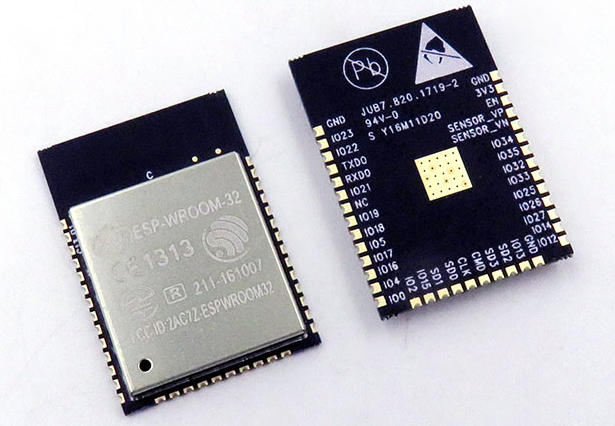
\includegraphics[width=0.6\linewidth]{Imagenes/esp32-wroom-s32-00}
\end{figure}

\subsubsection{Control de potencia AC por ángulo de fase}

``Los SCR y los TRIAC, permiten aplicar una técnica muy conveniente y eficaz para controlar el voltaje promedio y por lo tanto la potencia aplicada a una carga, cambiando el ángulo de fase con el cual la fuente de voltaje se aplica a ésta, tal como se muestra en la figura \ref{fig:triacgraph}. Esta técnica de control de voltaje es muy usada en las aplicaciones de regulación de motores, iluminación y temperatura, por ser el voltaje la variable principal en estos tres procesos''.\cite{CEKIT}\\


\begin{figure}[!t]
	\centering
	\caption{Representación gráfica del ángulo de disparo y de conducción del TRIAC y de la carga. Tomado de: \cite{CEKIT}.}
	\label{fig:triacgraph}
	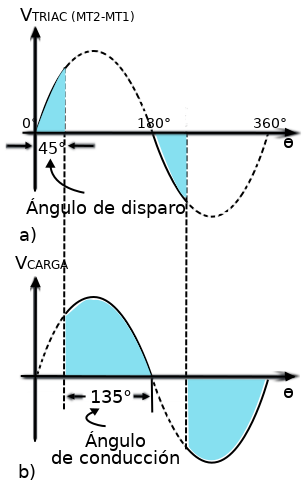
\includegraphics[width=0.4\linewidth]{Imagenes/TRIAC_graph}
\end{figure}

\subsubsection{Control de Cargas DC}

Los transistores como switch permiten controlar las cargas de corriente continua típicas como los motores y LED's, a parte de poder funcionar en dos estados, encendido y apagado Este control se da mediante la modulación por ancho de pulso (PWM), ya que al variar el ancho de pulso de la señal eléctrica se modifica la cantidad de energía entregada a la carga, tal como se muestra en la figura \ref{fig:pwm-duty-800x396}. \cite{PWM}\\

\begin{figure}[!t]
	\centering
	\caption{Ciclo Útil PWM. [Imagen Propia] }
	\label{fig:pwm-duty-800x396}
	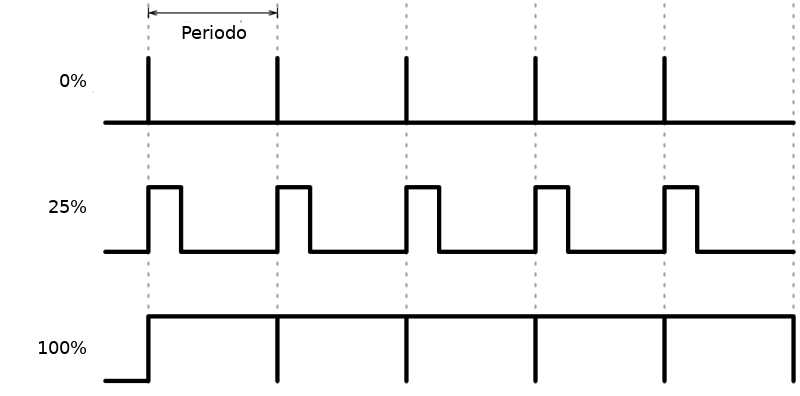
\includegraphics[width=0.6\linewidth]{Imagenes/pwm}
\end{figure}

\subsection{Software}

\subsubsection{ESP-IDF}

ESP-IDF es el entorno de desarrollo oficial para el ESP32 desarrollado por Espressif System, el cual mediante una serie de comandos específicos escritos en la terminal (en el caso de linux), habilita la configuración del ESP32 en cuanto a su funcionamiento, es decir, permite encender o apagar características como el WiFi, el Bluetooth o realizar particiones de memoria, ademas de esto, se puede cargar el código por el puerto USB al ESP32, al igual que visualizar la información generada por el ESP32 por el mismo puerto. \cite{ES}\\
\section{Desarrollo}
\subsection{Hardware}\label{sec:hw}

El prototipo para Smart House está equipado con etapas de potencia de corriente alterna y directa, etapa de adquisición de datos, entre otras características que permitan cumplir con los objetivos planteados. Este fue Diseñado en el software Proteus, desde el esquemático hasta la placa de circuito impreso (PCB), en la figura \ref{fig:esp32} se observa el esquematico de la tarjeta ESP32 construido junto con su distribución de pines, además de sus conexiones correspondientes dentro de este programa. El prototipo está separado en dos secciones, la etapa de potencia AC y la etapa DC, en la última, se encuentra la mayor parte de circuitos que funcionan con corriente directa.\\

%\begin{figure}[H]
%	\centering
%	\caption{ESP32 creado en proteus [Imagen Propia]}
%	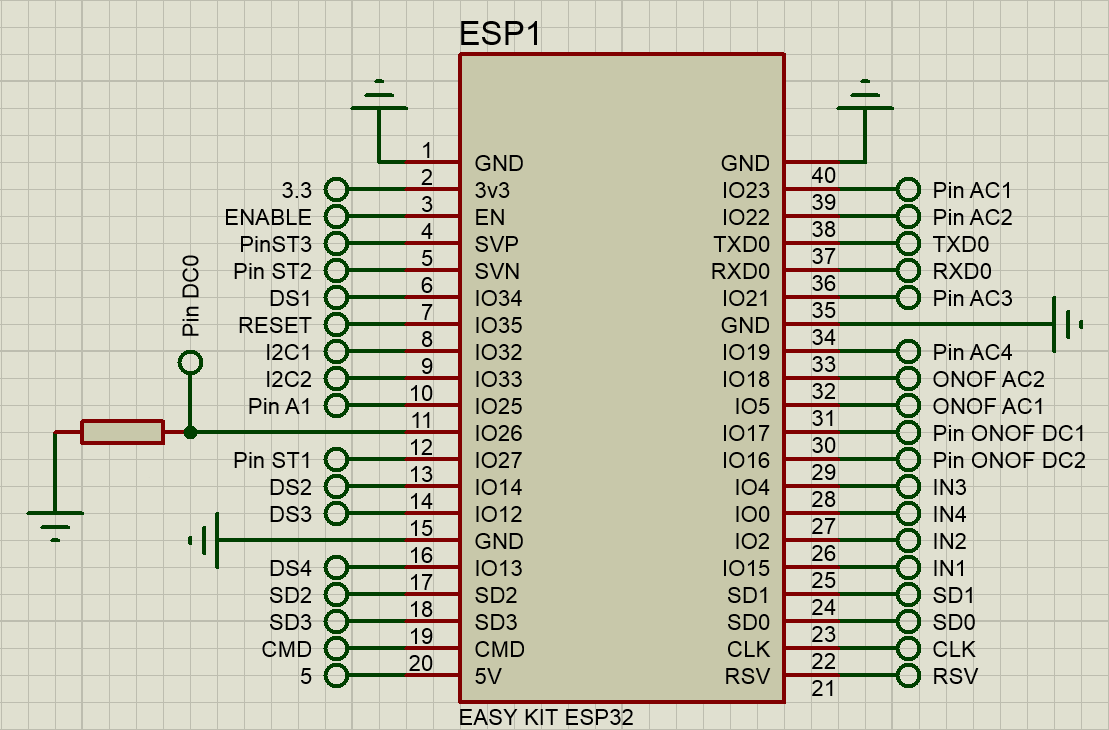
\includegraphics[width=0.5\linewidth]{Imagenes/ESP32}	
%	\label{fig:esp32}
%\end{figure}

En los siguientes ítems se resaltaran las características más importantes que lleva el circuito:\\

	\subsubsection{Alimentacion}
	
	\paragraph{Corriente alterna (AC)}
		El prototipo recibe el voltaje directamente de la red eléctrica a la que se encuentra conectado el entorno de aplicación, para el caso de Colombia, la red doméstica comúnmente otorga 110V AC, los cuales son regulados para el funcionamiento adecuado del prototipo, como la etapa de potencia AC y el detector de cruce por cero con el fin de sincronizar la tarjeta a dicha red eléctrica.\\
		
	\paragraph{Corriente directa (DC)}
		Para la alimentación DC del circuito se hace uso de un conversor AC-DC que regula el voltaje de la red eléctrica a 12V DC y 2A, con los cuales se manejara la etapa de potencia DC, además de ser usados por dos modulos conversores DC-DC, ambos con entradas de 12V DC y con salidas a los niveles lógicos comunes, 5V y 3.3V, empleados con el fin de alimentar dispositivos como opto acopladores, transistores BJT o relevadores con activación de 5V, así como también la tarjeta de prototipo ESP32.\\
			
%		\begin{figure}[H]
%			\centering
%			\caption{Modulo conversor DC-DC. Tomado de: \cite{DCDC}}
%			\label{fig:DCDC}
%			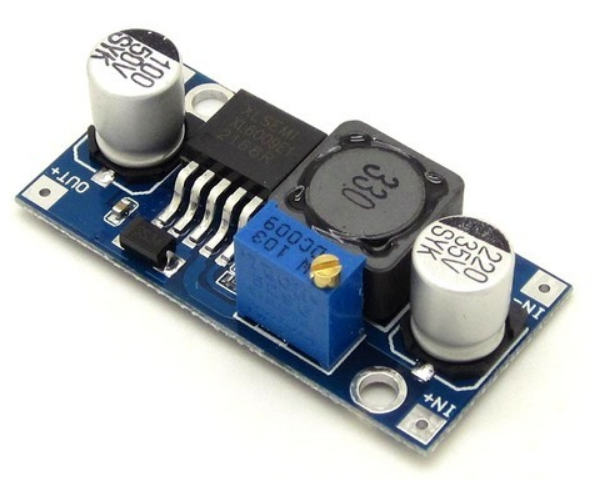
\includegraphics[width=0.5\linewidth]{Imagenes/DCDC}
%		\end{figure}
	
	\subsubsection{Entradas}
	\paragraph{Sensores}
		el prototipo viene equipado con una etapa de adquisición de datos con capacidad entre 7 a 134 sensores, pues posee una entrada I2C, ampliando el número de dispositivos conectados, lo cual también permitiría adicionar tareas más específicas en escenarios que lo requieran.\\
		
	 	Teniendo en cuenta que el ESP32 funciona en voltajes lógicos de 3.3V, se tienen 4 entradas de sensores directamente conectados a los pines de la tarjeta, con la capacidad de cambiar el voltaje de alimentación para 3 de ellos, pues en el mercado se encuentran sensores que manejan voltajes de alimentación ya sea de 3.3V o 5V, mientras que la cuarta entrada se encuentra alimentada con 5V para un sensor analogico, esta viene acondicionada con un diodo zener en contraposición, para evitar que la tarjeta ESP32 tenga un voltaje de entrada superior a 3.3V.\\
		
		Las tres entradas para sensores de estado, a diferencia de las demás, se encuentran conectadas a pines de la tarjeta que no presentan resistencia de pull down por software, por ello se agregan estas dentro del hardware del sistema.\\
		
%		\begin{figure}[H]
%			\centering
%			\caption{Entrada de sensores[Imagen Propia]}
%			\label{fig:SVS}
%			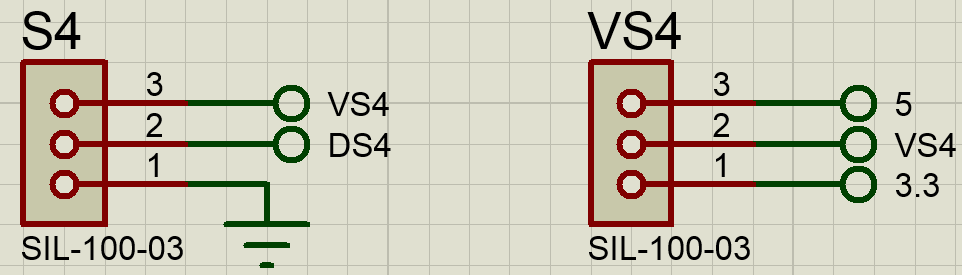
\includegraphics[width=0.7\linewidth]{Imagenes/SVS}
%		\end{figure}
%	
%		\begin{figure}[H]
%			\centering
%			\caption{Entrada para sensor de calidad de aire[Imagen Propia]}
%			\label{fig:S1Aire}
%			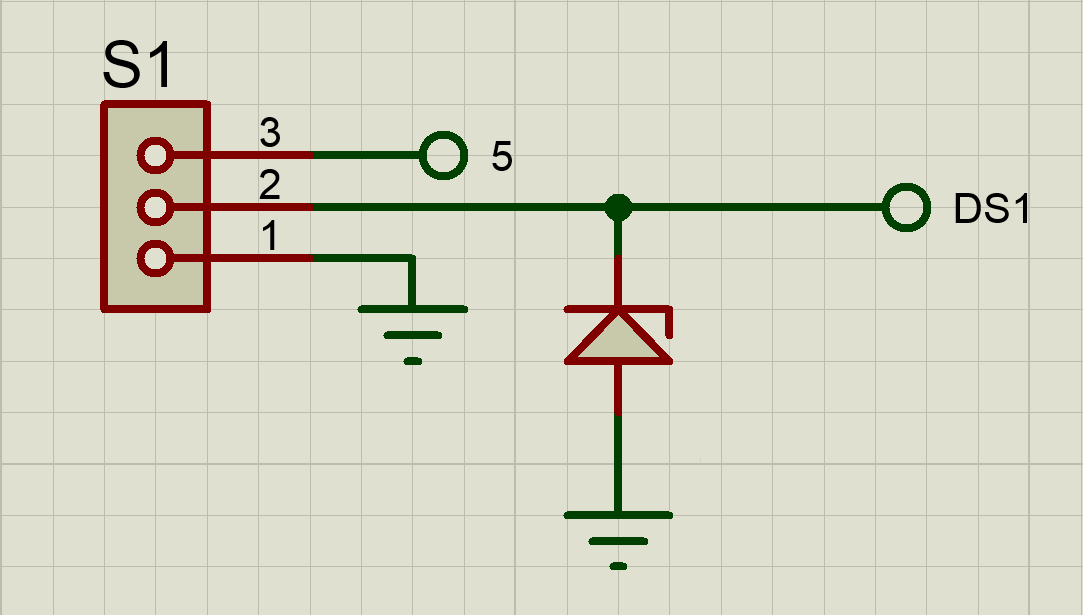
\includegraphics[width=0.6\linewidth]{Imagenes/S1Aire}
%		\end{figure}
%	
%		\begin{figure}[H]
%			\centering
%			\caption{Entrada para sensores con resistencia de pull down[Imagen Propia]}
%			\label{fig:ST}
%			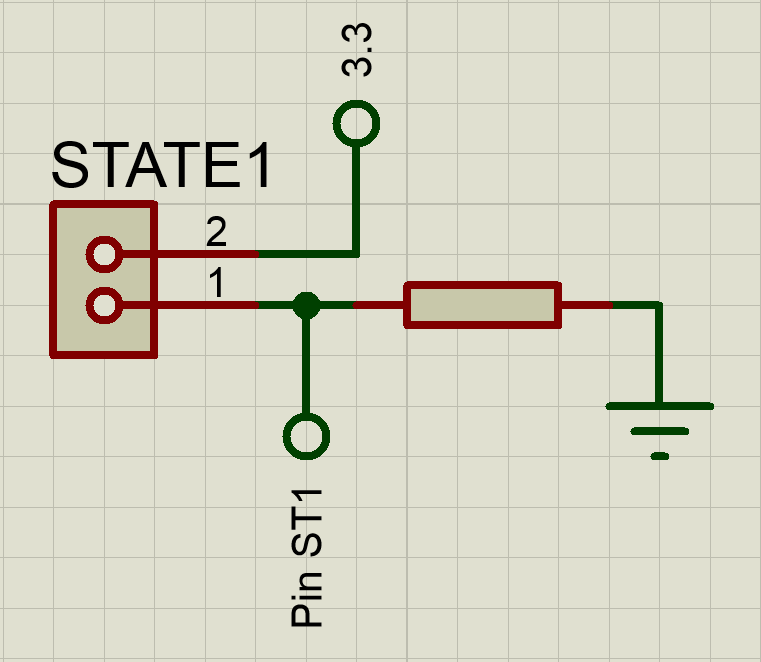
\includegraphics[width=0.5\linewidth]{Imagenes/ST}
%		\end{figure}		
	
	\paragraph{Interacción con el sistema}
		Para calibrar la salida audible se hace uso de una resistencia variable (Potenciometro), el cual permite regular el voltaje de entrada al circuito de amplificación que será descrito en el presente capitulo en la sección de salidas del hardware.\\
		
		Presionando el botón enable se reinicia la tarjeta ESP32, junto con su firmware.\\
		
		Presionando el botón reset se borran las credenciales ingresadas para la conexión del ESP32 a la red wifi.\\
	
		
	\subsubsection{Salidas:}
	\paragraph{Etapa de potencia AC}
		Se encuentra diseñada a una potencia de 2000W en un total de seis cargas, cuatro de ellas cuentan con un circuito para el control por ángulo de fase, como se observa en la figura \ref{fig:CAC1}, con una capacidad individual de 500W, gracias a el TRIAC BTA26600, el cual soporta una corriente máxima de 25A; con el fin de proteger el ESP32, se hace uso de optoacopladores MOC3021, debido a su funcionalidad de aislar circuitos de forma óptica.\\
		
%		\begin{figure}[H]
%			\centering
%			\caption{Control por angulo de fase [Imagen Propia]}
%			\label{fig:CAC1}
%			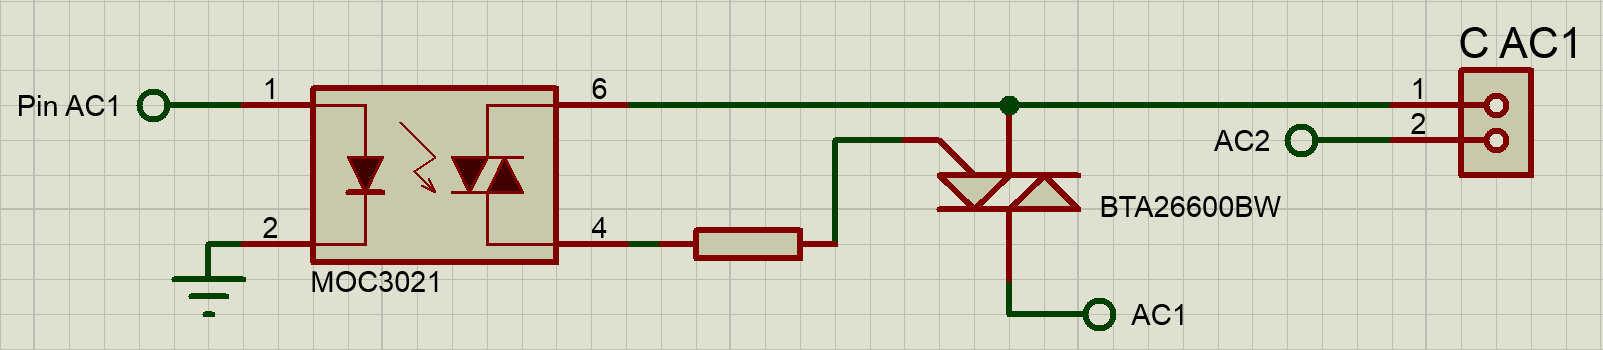
\includegraphics[width=0.8\linewidth]{Imagenes/CAC1}
%		\end{figure}
%	
%		\begin{figure}[H]
%			\centering
%			\caption{Triac BTA26600. Tomado de: \cite{TRIAC}}
%			\label{fig:TRIAC}
%			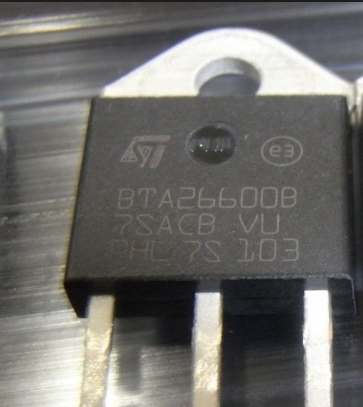
\includegraphics[width=0.35\linewidth]{Imagenes/TRIAC}
%		\end{figure}
%	
		Las dos cargas restantes corresponden a un sistema de encendido y apagado, cuyo funcionamiento se basa en un relevador SRA-05VDC-CL activado a 5V por medio de un transistor BJT como switch, gracias a este relé, las salidas tienen capacidad de hasta 200W cada una, en la figura \ref{fig:ONOFAC} se observa el circuito diseñado en proteus. Para proteger el ESP32 el prototipo se vale de ese dispositivo, puesto que presenta un aislamiento magnético por la naturaleza de su operación.\\
	
%		\begin{figure}[H]
%			\centering
%			\caption{Interruptor para cargas AC [Imagen Propia]}
%			\label{fig:ONOFAC}
%			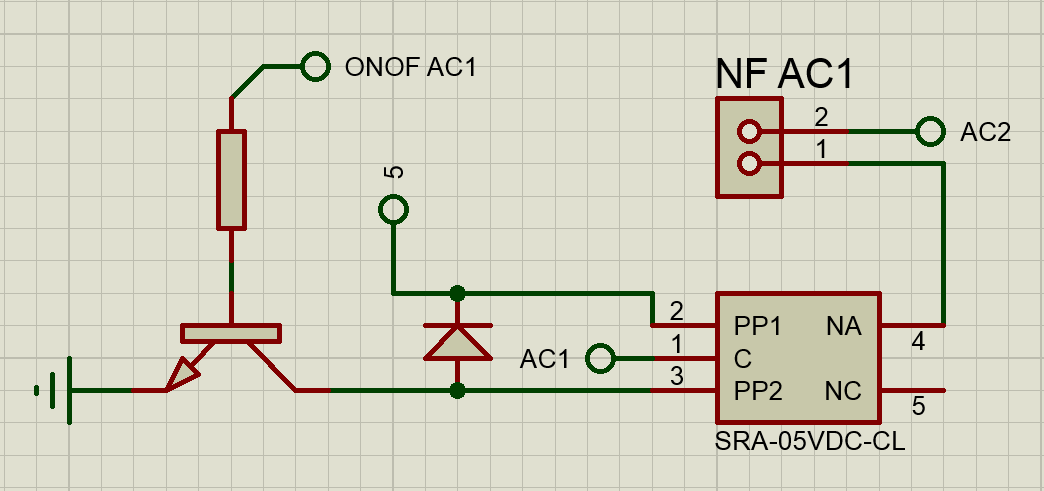
\includegraphics[width=0.7\linewidth]{Imagenes/ONOFAC}
%		\end{figure}
	
		Dentro de la etapa AC se encuentra el detector de cruce por cero, el cual se vale de un fototransistor 4N25, debido a su alta capacidad de aislamiento, tomando la onda rectificada completa y pasándola a un nivel lógico de 3.3V, esta parte del circuito se observa en la figura \ref{fig:DC01}; para que la señal sea más confiable se hace uso de un Schmitt-Trigger CD40106 mostrado en la figura \ref{fig:DC02}, valiéndose de la histéresis de voltaje garantizando que la señal de salida sea poco susceptible al ruido \cite{DC0}.\\
		
%		\begin{figure}[H]
%			\centering
%			\caption{Detector de cruce por cero [Imagen Propia]}
%			\label{fig:DC01}
%			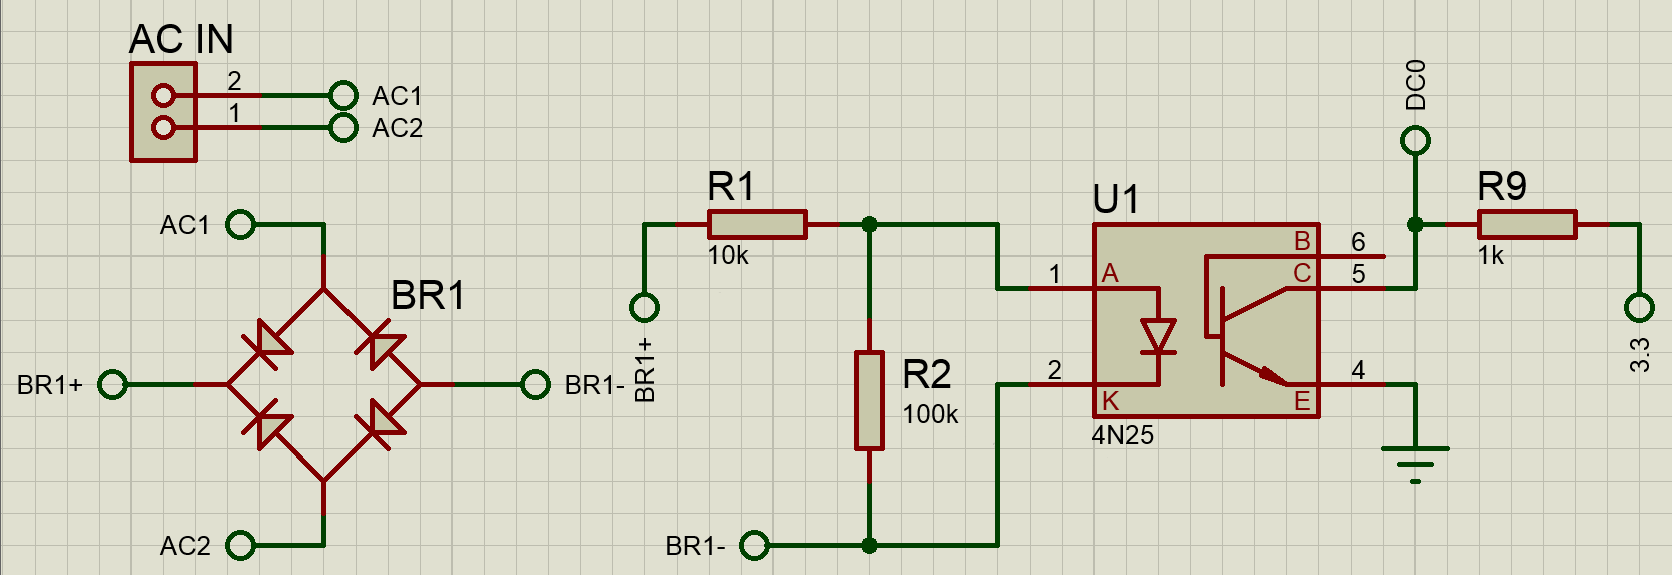
\includegraphics[width=0.85\linewidth]{Imagenes/DC01}
%		\end{figure}
%	
%		\begin{figure}[H]
%			\centering
%			\caption{Schmitt trigger para el detector de cruce por cero [Imagen Propia]}
%			\label{fig:DC02}
%			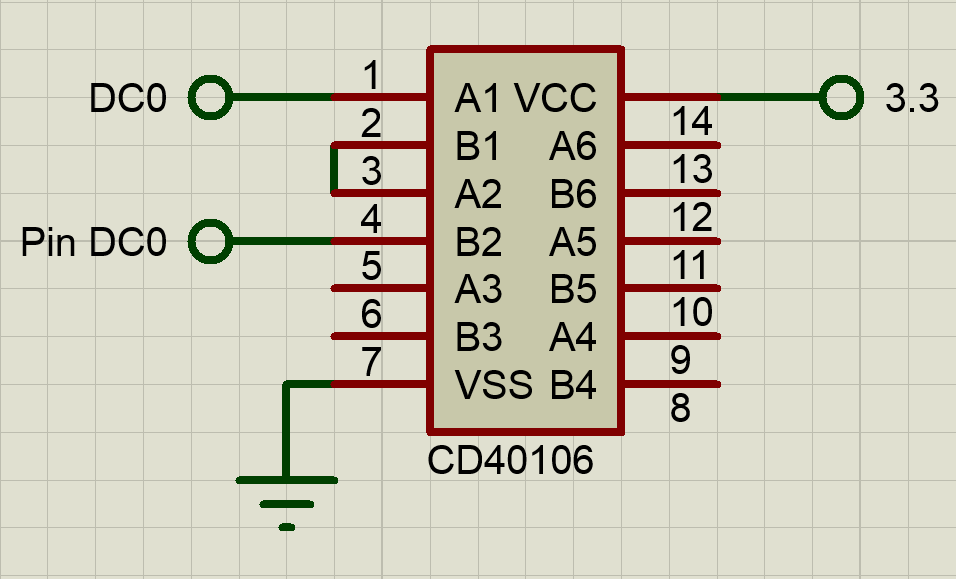
\includegraphics[width=0.5\linewidth]{Imagenes/DC02}
%		\end{figure}
	
	\paragraph{Etapa DC}
		esta etapa cuenta con cuatro salidas de control diseñadas para cargas de 12V, de las cuales, dos de ellas tienen un enfoque enfoque a motores, puesto que está equipada con control de velocidad a base de PWM e inversión de giro con un puente h usando transistores mosfet IRLZ44N; el puente h se encuentra controlado por un circuito integrado L293D, que garantiza un voltaje Vgs adecuado para la correcta activación del los transistores del puente h; este circuito se muestra en la figura \ref{fig:L293D} y \ref{fig:CDC}.\cite{IRL}.\\
		
		Las dos salidas restantes también cuentan con mosfet IRLZ44N, y su control igualmente es a base de PWM, mas no permite realizar la inversión de giro, por lo cual se enfoca a dispositivos como lámparas LEDs, el diseño en proteus se muestra en la figura \ref{fig:ONOFDC}.\\
		
%		\begin{figure}[H]
%			\centering
%			\caption{Integrado L293D [Imagen Propia]}
%			\label{fig:L293D}
%			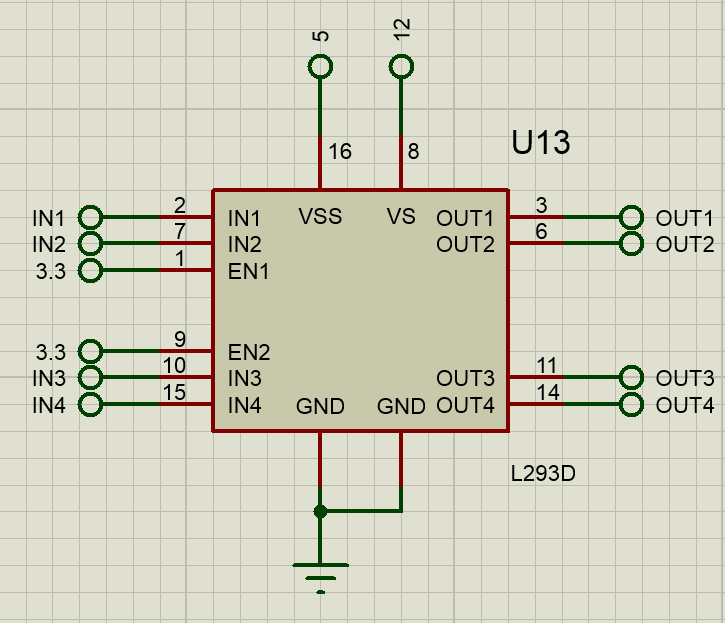
\includegraphics[width=0.5\linewidth]{Imagenes/L293D}
%		\end{figure}
%		
%		\begin{figure}[H]
%			\centering
%			\caption{Puente h para control de motores DC [Imagen Propia]}
%			\label{fig:CDC}
%			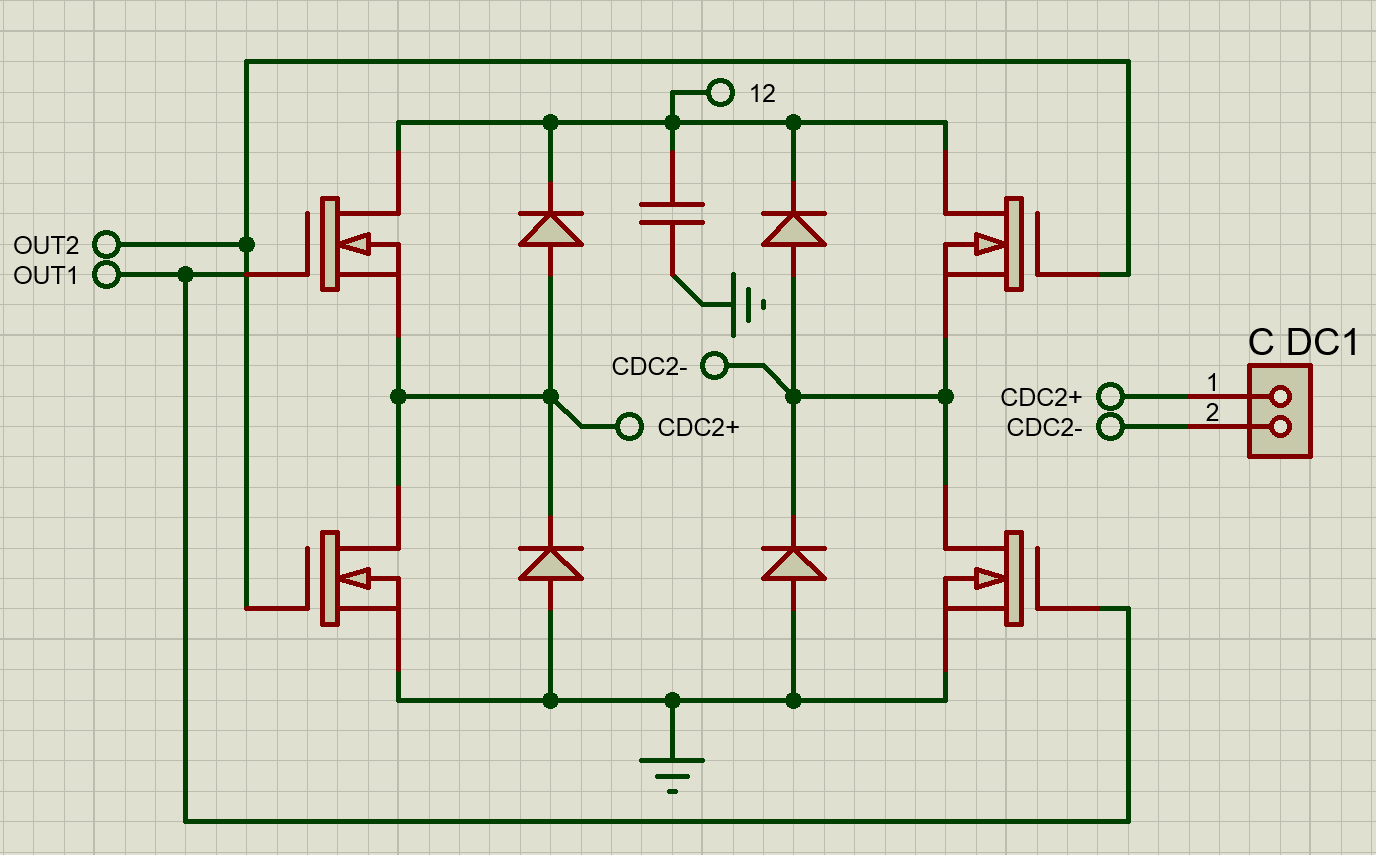
\includegraphics[width=0.7\linewidth]{Imagenes/CDC}
%		\end{figure}
%	
%		\begin{figure}[H]
%			\centering
%			\caption{Control para cargas DC [Imagen Propia]}
%			\label{fig:ONOFDC}
%			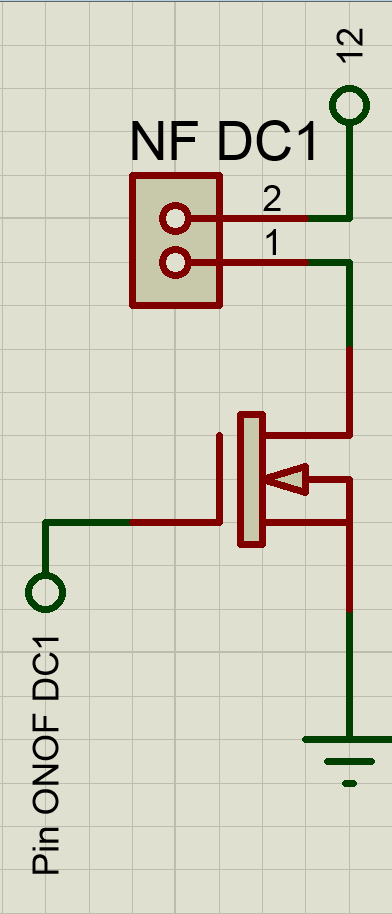
\includegraphics[width=0.25\linewidth]{Imagenes/ONOFDC}
%		\end{figure}
	
	\paragraph{Salida audible}
		está diseñada para emitir desde sonidos a una sola frecuencia, o sonido mono estéreo, caso dado cuando se activa una regla programada en la aplicación web, enfocada a las cargas de encendido y apagado, tanto de la etapa de potencia AC como la etapa DC; el sonido emitido por el prototipo corresponde a una voz con tonalidad femenina, pronunciando el estado en el cual se configura la carga según la regla (ya sea encendido, o apagado).\\
		
		El circuito utilizado para la salida audible está basado en el amplificador de audio LM386, implementando el esquema típico de aplicación ilustrado en su datasheet \cite{LM386}, en la figura \ref{fig:AUD} se observa implementado en el software proteus.
		
		
%		\begin{figure}[H]
%			\centering
%			\caption{Circuito tipico para el LM386 [Imagen Propia]}
%			\label{fig:AUD}
%			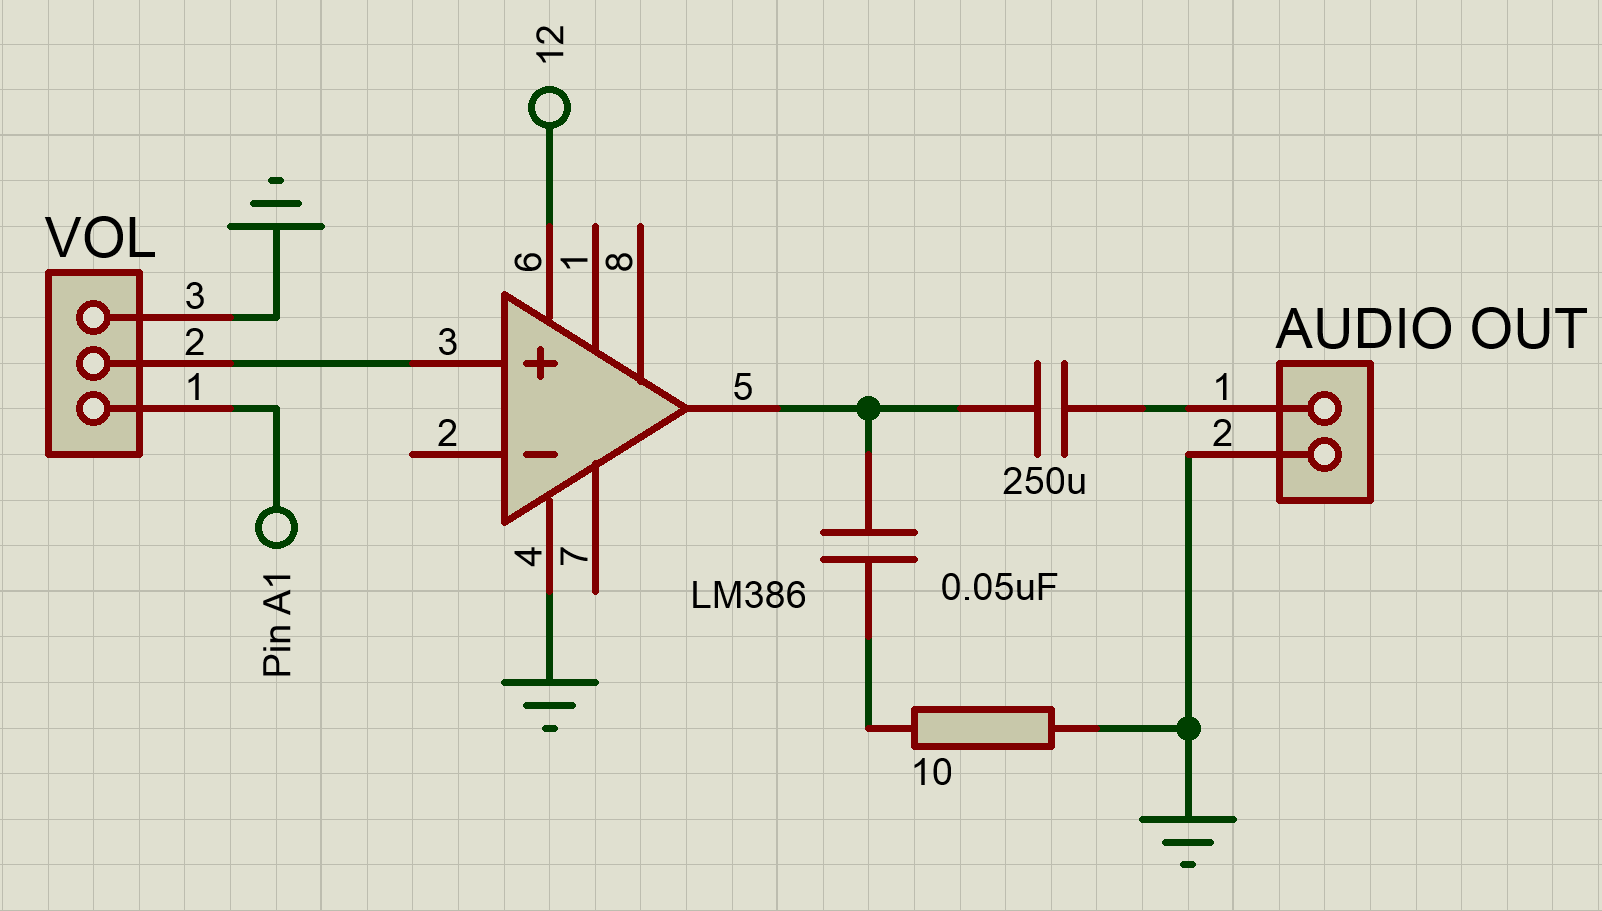
\includegraphics[width=0.7\linewidth]{Imagenes/AUD}
%		\end{figure}		
				
\subsection{Firmware}

El firmware se desarrolla sobre el framework o SDK oficial de Espressif Systems, ESP-IDF el cual posee una documentación \cite{ES} muy útil a la hora de utilizar las diferentes APIs presentes en este; para el desarrollo de la aplicación es necesario contar con los requisitos que se observan en la figura \ref{fig:what-you-need}. El framework incluye un kernel de tiempo real llamado FreeRTOS, el cual da soporte al manejo de los diversos recursos del sistema; al ser un RTOS, las funciones se definen mediante tareas, entonces cada funcionalidad de la tarjeta o grupo de funcionalidades se desarrolla en una o varias tareas que realicen las acciones adecuadas.

%\begin{figure}[H]
%	\centering
%	\caption{ESP-IDF. Tomado de: \cite{ES}}
%	\label{fig:what-you-need}
%	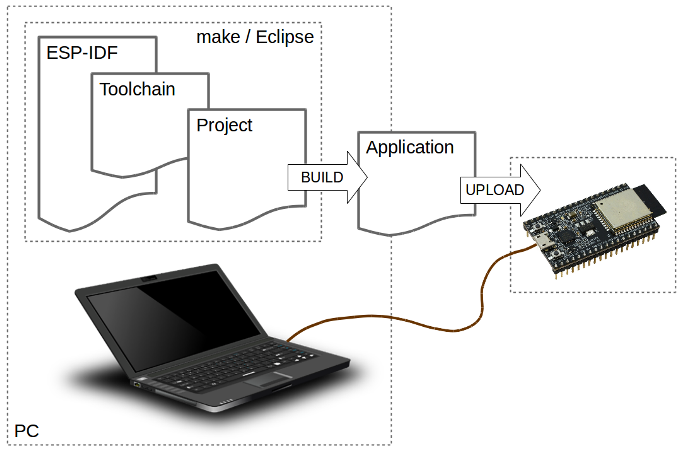
\includegraphics[width=0.5\linewidth]{Imagenes/what-you-need}
%\end{figure}

\subsection{Software}

En esta sección se desarrolla una aplicación web, la cual se encarga de ejecutar la gestión entre el usuario y la tarjeta. De este modo, se usa un patrón de arquitectura Modelo-Vista-Controlador (MVC). Aquel modelo es realmente útil ya que separa la lógica de negocio de la interfaz de usuario, incrementando la reutilización y flexibilidad, además la escalabilidad de ambos aspectos por separado, dicho esto la aplicación cuenta con diferentes modelos, controladores y vistas \cite{MVC1}. La función de cada parte de esta arquitectura se puede observar en la figura \ref{fig:mvc}.\\

%\begin{figure}[H]
%	\centering
%	\caption{Modelo-Vista-Controlador [Imagen Propia]}
%	\label{fig:mvc}
%	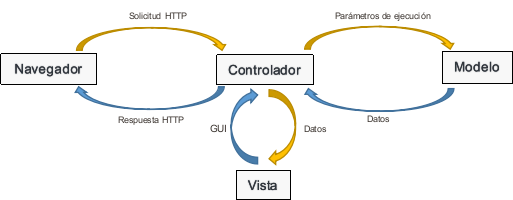
\includegraphics[width=0.7\linewidth]{Imagenes/MVC}
%\end{figure}

Además, con este framework se hace uso de un ORM (Mapeo Objeto-Relacional) llamado Eloquent. Esta es una forma de mapear los datos que se encuentran en la base de datos a objetos de PHP y viceversa, esto facilita el uso de diferentes gestores de bases de datos como MySQL, SQLite, entre otras, ya que todas las consultas estan en PHP y el ORM ya se encarga del mapeo a los comandos SQL como se observa en la figura \ref{fig:orm}. Eloquent usa los modelos para enviar y recibir información de la base de datos\cite{Eloq}.

%\begin{figure}[H]
%	\centering
%	\caption[ORM]{ORM [Imagen Propia]}
%	\label{fig:orm}
%	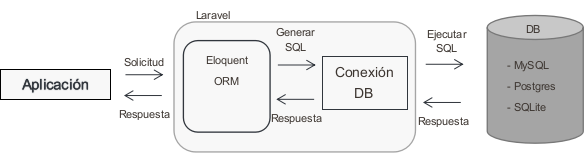
\includegraphics[width=0.7\linewidth]{Imagenes/ORM}
%\end{figure}

\subsection{Prueba Beta}

Esta prueba se desarrolla en el entorno del cliente o usuario, arrojando resultados sobre las funcionalidades provistas para el software, además de dar la aceptación por parte del cliente si el producto funciona de manera adecuada o esperada \cite{PB}. Con el fin de realizar dicha vereficación se analizan los objetivos a cumplir y los alcances, por lo tanto se separan los casos de prueba con el propósito de formular las preguntas que deben contestar las personas. las preguntas formuladas para estos se encuentran en el Anexo \ref{AnexoB}.\\

\paragraph{Prueba de conectividad de la tarjeta:} en la cual la persona que participa en esta prueba debe realizar los primeros pasos para conectar la tarjeta con internet como se expone más adelante en resultados y se explica en Anexos en el manual de usuario.\\

\paragraph{Prueba de la Aplicación Web:} en la cual se evalúan diferentes aspectos y la mas extensa, ya que se evalúa el inicio de sesión, el monitoreo y control de todos los dispositivos que se encuentra conectados en tarjeta SmartHouse, además de las funcionalidades que posee el sistema en general.
\section{Resultados y Análisis}

En este capitulo se describen ciertos pasos y funcionamientos de la solución en general. En la figura \ref{fig:iot} esta el esquema del sistema IoT.\\

\begin{figure}[!t]
	\centering
	\caption{Esquema Solución SmartHouse [Imagen Propia]}
	\label{fig:iot}
	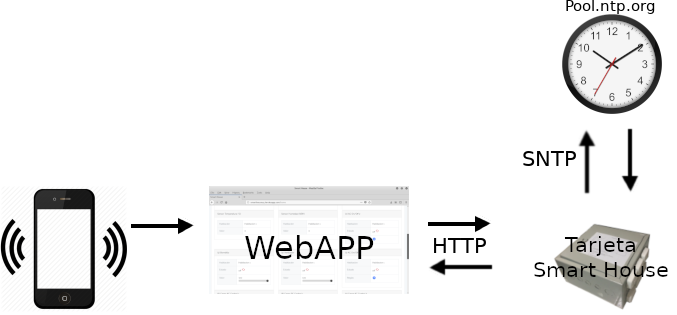
\includegraphics[width=0.8\linewidth]{Imagenes/IOT}
\end{figure}

\subsection{Software}

 La aplicación web se encuentra compuesta por los siguientes sitios y las diferentes interacciones basadas en las funciones básicas, crear, leer, actualizar y borrar (CRUD).\\

\begin{itemize}
	\item Parte Pública
	\item Parte Privada
	\begin{itemize}
		\item API
		\item Panel de Control
		\begin{itemize}
			\item Crear
			\item Ver
			\item Editar
			\item Eliminar 
		\end{itemize}
	\end{itemize}
\end{itemize}

De acuerdo con la lista anterior, se toman en cuenta dos partes, una pública y una privada, como se observa en la figura \ref{fig:index}. En la parte pública se encuentra una vista con la información de contacto del fabricante, solicitudes de registro o productos y la cantidad de usuarios que actualmente estan registrados en la aplicación. En la parte privada se encuentra la interacción de los usuarios sea administrador, dueño de una casa o de una habitación, para controlar y observar sus datos.\\

\begin{figure}[!t]
\centering
\caption{Página de Inicio. [Imagen Propia]}
\label{fig:index}
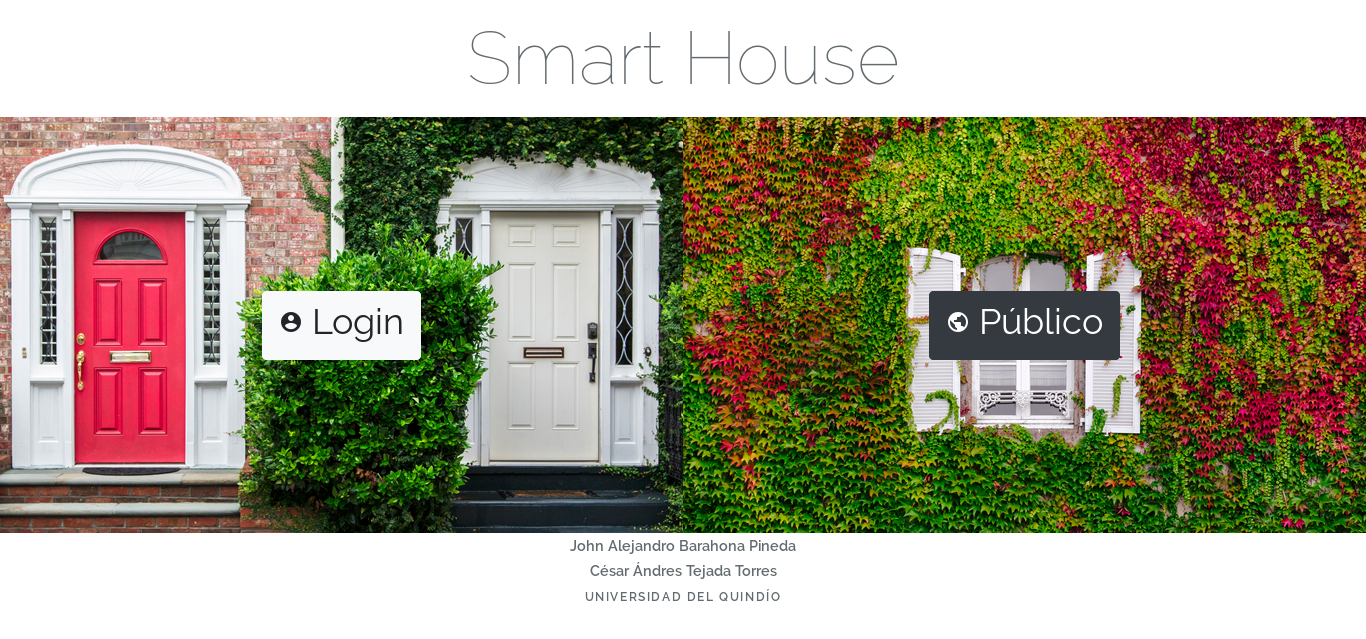
\includegraphics[width=0.9\linewidth]{Imagenes/Index}
\end{figure}

\subsubsection{Parte Pública}

En esta vista únicamente hay opciones para el contacto y solicitudes, como se menciona anteriormente, es sencilla debido a la poca información que contiene.

\subsubsection{Parte Privada}

En primera instancia, un usuario administrador tiene la posibilidad de crear, ver, editar y eliminar los registros de la aplicación, la vista de este usuario se puede observar en la figura \ref{fig:views}\textbf{(a)}. También existe el usuario dueño de la vivienda, este puede revisar y editar algunos campos de sus usuarios hijos o usuarios habitación,  en la figura \ref{fig:views}\textbf{(b)} se observa su vista. Por último, se tiene el usuario habitación que únicamente visualiza los datos  del cuarto en cuestión, según se observa en la figura \ref{fig:views}\textbf{(c)}, por tal motivo el panel de control muestra una vista general de los datos y el estado de sus dispositivos, además de tener la capacidad de editar partes básicas de su habitación y perfil.\\

Adicionalmente, si el usuario desea añadir, modificar o eliminar una regla, puede lograrlo mediante el botón de reglas en el panel de control, el cual lo redirige a una página que indica una hora de inicio y finalización en la que el bombillo led enciende y apaga respectivamente. \\

\begin{figure}[!t]
	\centering
	\caption{Vistas de Usuarios [Imagen Propia]}
	\label{fig:views}
	\subfigure[Usuario Administrador]{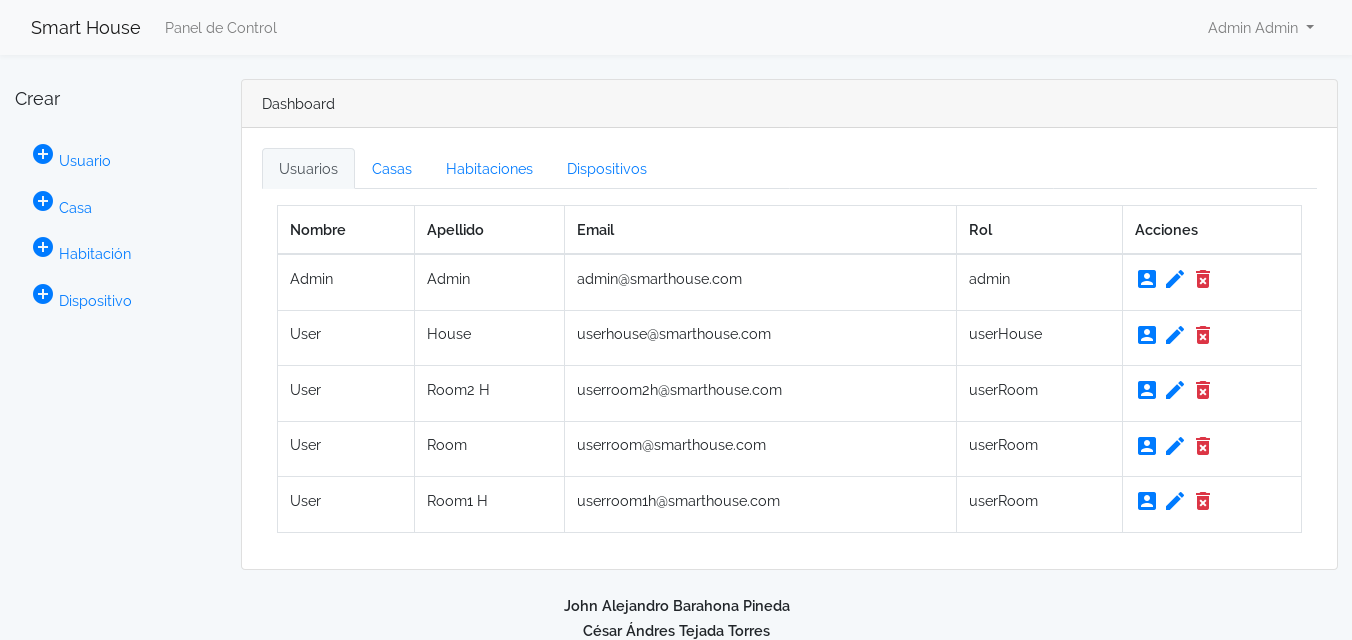
\includegraphics[width=0.9\linewidth]{Imagenes/Admin_view}}
	\subfigure[Usuario de Casa]{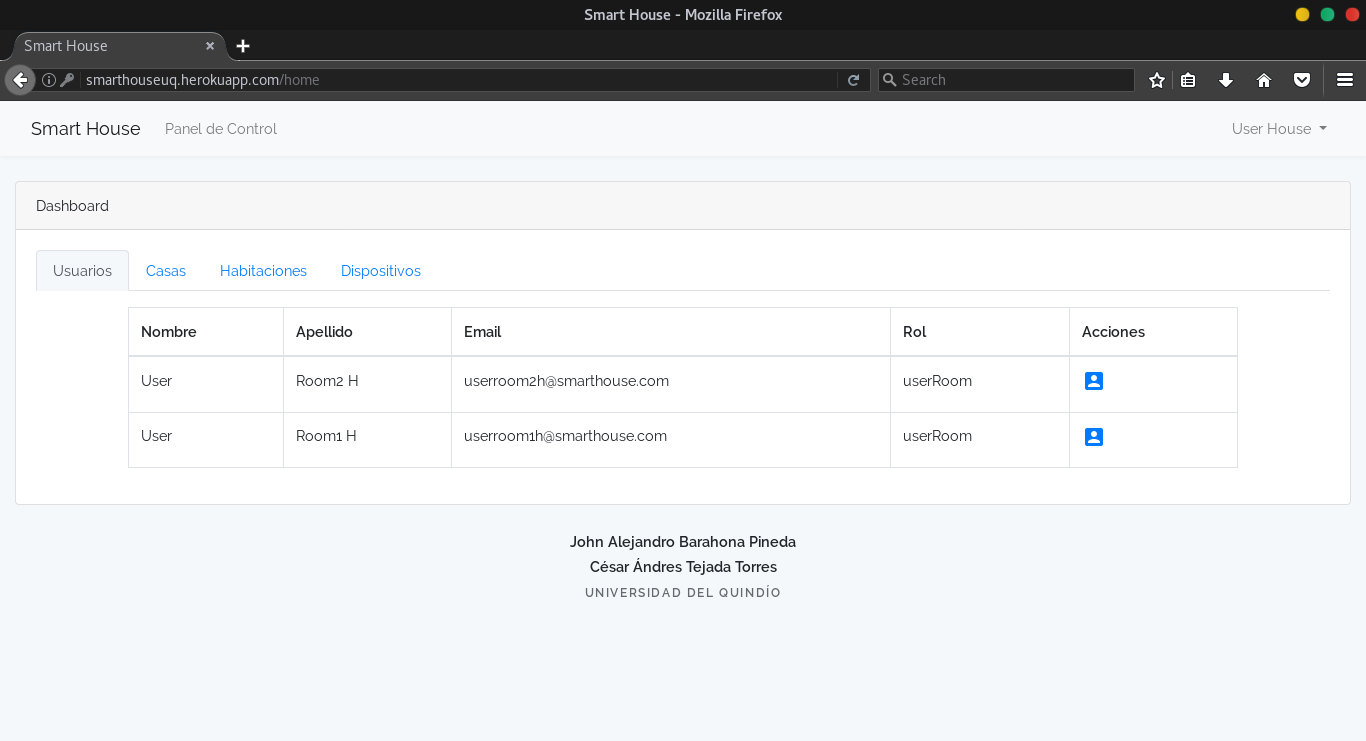
\includegraphics[width=0.45\linewidth]{Imagenes/UserH_view}}
	\subfigure[Usuario de Habitación]{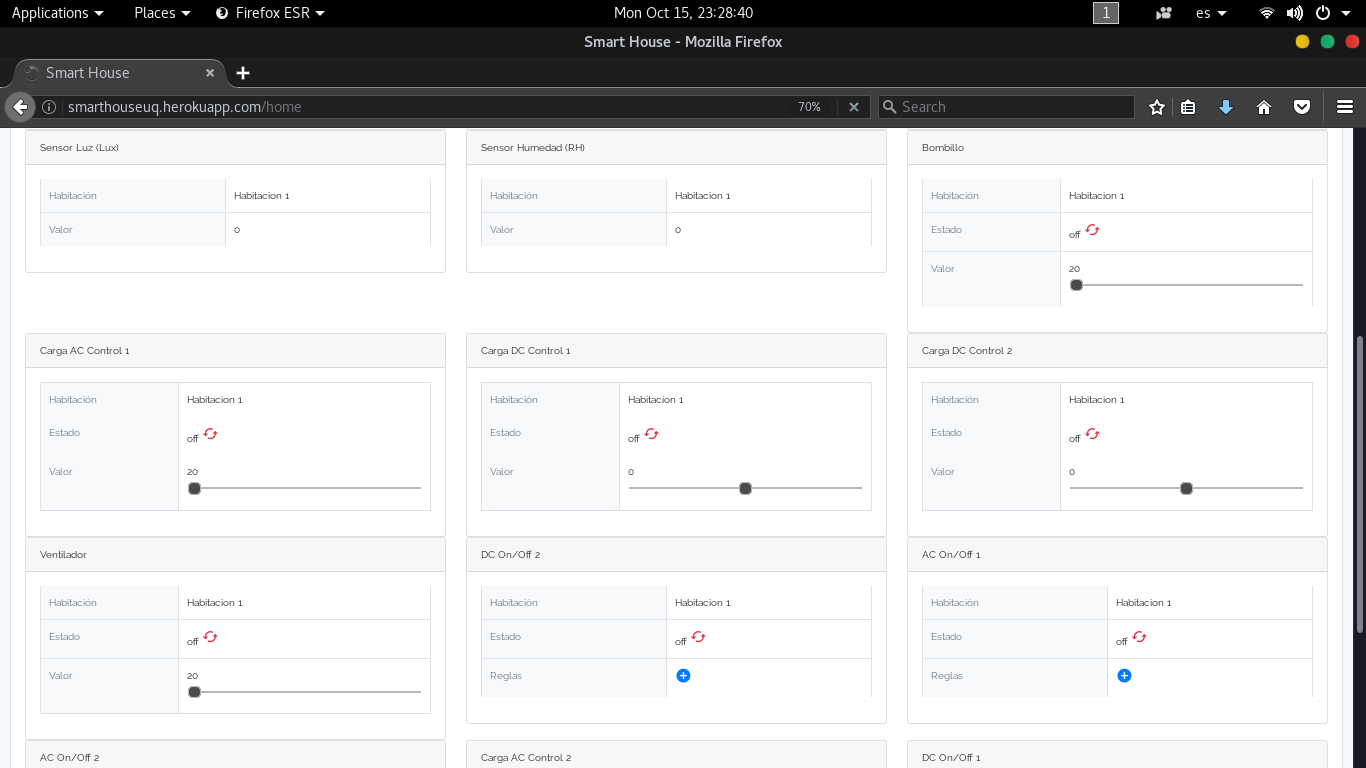
\includegraphics[width=0.45\linewidth]{Imagenes/UserR_view}}
\end{figure}

\subsubsection{Base de Datos}

La estructura de la base de datos se puede observar en la figura \ref{fig:db}, aquí se observan los diferentes campos que posee cada tabla, además de las llaves y sus relaciones, las relaciones presentes en esta estructura son de tipo 1:N, es decir, por ejemplo un usuario puede tener relacionadas N casas.\\  

\begin{figure}[!t]
\centering
\caption{Base de datos SmartHouse [Imagen Propia]}
\label{fig:db}
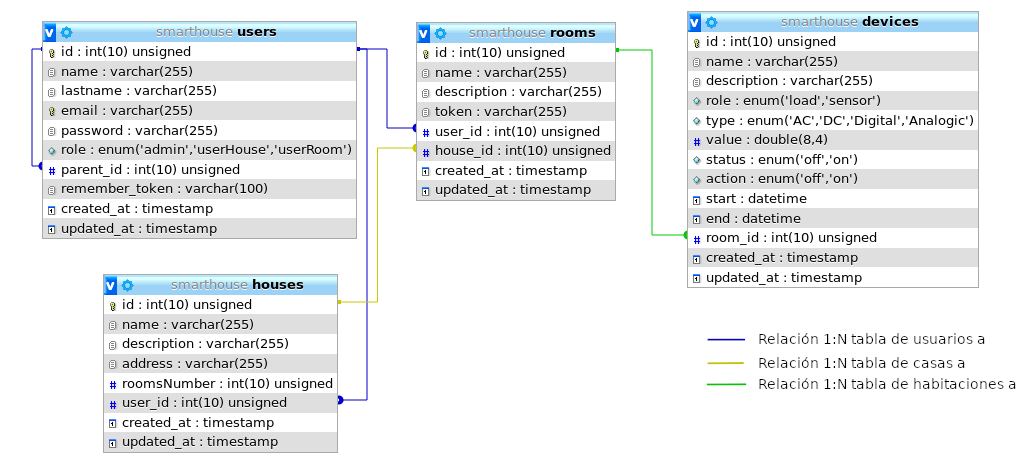
\includegraphics[width=0.8\linewidth]{Imagenes/DB}
\end{figure}

Las diversas interfaces generadas en la aplicación, permiten el monitoreo, control y la interacción del usuario con el dispositivo presente en su habitación, haciendo posible el cambio de estado de las salidas y así mismo visualizar los datos producidos por los sensores. También cabe resaltar que algunas salidas tienen la posibilidad de automatizarse a través de reglas, es decir, indicarle en que momento encender o apagar cierto dispositivo que se encuentre conectado a la tarjeta como se ha mencionado. Por otra parte, todos los datos generados de la interacción del cliente con el programa se almacenan en la base de datos enlazada a dicha aplicación permitiendo una gestión adecuada de estos. Los resultados obtenidos del diseño de este software cumplen con el objetivo a partir del cual se construye y también se tienen algunas funciones adicionales como los usuarios administradores de casa, esto asegurando la escalabilidad de la aplicación. \\

\subsection{Firmware}

El firmware se encuentra compuesto, como se ha mencionado anteriormente, de tareas, en la figura \ref{fig:tareas} se observa un bosquejo del trabajo de las diferentes tareas de las que se compone este, tomando por función principal la encargada de gestionar la conexión a Wi-Fi y almacenar sus credenciales, dependiendo del estado de si están almacenadas o no, el sistema se comporta de una u otra forma.\\

\begin{figure}[!t]
	\centering
	\caption{Esquema de Tareas [Imagen Propia]}
	\label{fig:tareas}
	
\includegraphics[width=0.8\linewidth]{Imagenes/tareas}
\end{figure}
 

\subsubsection{Escritura de Datos en la Aplicación Web}

Los datos que lee la tarjeta provienen de los diferentes sensores que tiene conectados, para la escritura de estos, en el firmware se desarrollan con varias tareas encargadas de leerlos y enviarlos a una tarea central. Los datos que están enviando contienen el id del dispositivo y la medida que lee en ese momento, estos se envían en forma de texto en formato JSON, organizándolos en la petición HTTP tipo GET; así la url que la tarjeta solicita, incluyendo el JSON de cada sensor, se observa en la figura \ref{fig:json}. La aplicación ya se encarga de almacenarlos y mostrarlos al usuario como se menciona anteriormente.\\

\begin{figure}[!t]
	\centering
	\caption{URL de la petición HTTP [Imagen Propia]}
	\label{fig:json}
	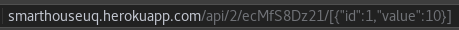
\includegraphics[width=0.9\linewidth]{Imagenes/JSON}
\end{figure}


\subsubsection{Lectura de Datos de Internet}

La tarjeta mantiene una actualización frecuente, para esto, cuando la tarjeta envía los datos de los sensores la aplicación responde con datos de cabecera HTTP, además de la información de los dispositivos que controla la tarjeta, esta los recibe en una cadena texto en formato JSON como se observa en la figura \ref{fig:httprqstesp}, los procesa y los dirige a las tareas pertinentes ya sea para encender o apagar algún dispositivo conectado a la tarjeta, también remite las reglas que el usuario ha definido.\\

\begin{figure}[!t]
	\centering
	\caption{Respues del la APP Web a la Tarjeta [Imagen Propia]}
	\label{fig:httprqstesp}
	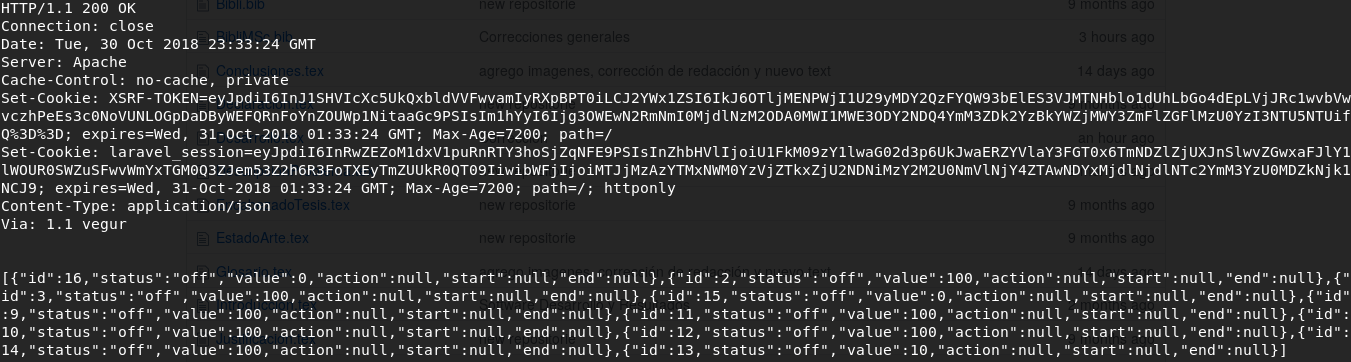
\includegraphics[width=0.9\linewidth]{Imagenes/HTTPRqstesp}
\end{figure}

Analizando los tiempos de resolución de la petición http, se tiene una media aproximada de 1s, el cual es un tiempo de respuesta aceptable dadas todas las funcionalidades provistas en el programa, aunque este tiempo varia, ya que el haber utilizado el puerto serie para observar estos resultados se agrega tiempo al procesamiento, así como también interfiere la velocidad en la conexión a internet y la señal de recepción de wi-fi.\\


\subsection{Hardware}

De acuerdo con los circuitos diseñados en la sección \ref{sec:hw}, en la figura \ref{fig:tarjeta} se observan las diferentes tarjetas ya ensambladas en una caja eléctrica para probar el funcionamiento del prototipo. Las salidas y entradas están distribuidas según lo propuesto e ilustradas en la caja eléctrica por medio de pegatinas, la figura \ref{fig:labels} muestra esta información; para las salidas AC se usan toma corrientes para conectar allí los diversos dispositivos, para las salidas DC se utilizan conectores hembra tipo banana para facilitar la conexión de estos dispositivos.\\

\begin{figure}[!t]
	\centering
	\caption{Tarjeta SmartHouse [Imagen Propia]}
	\label{fig:tarjeta}
	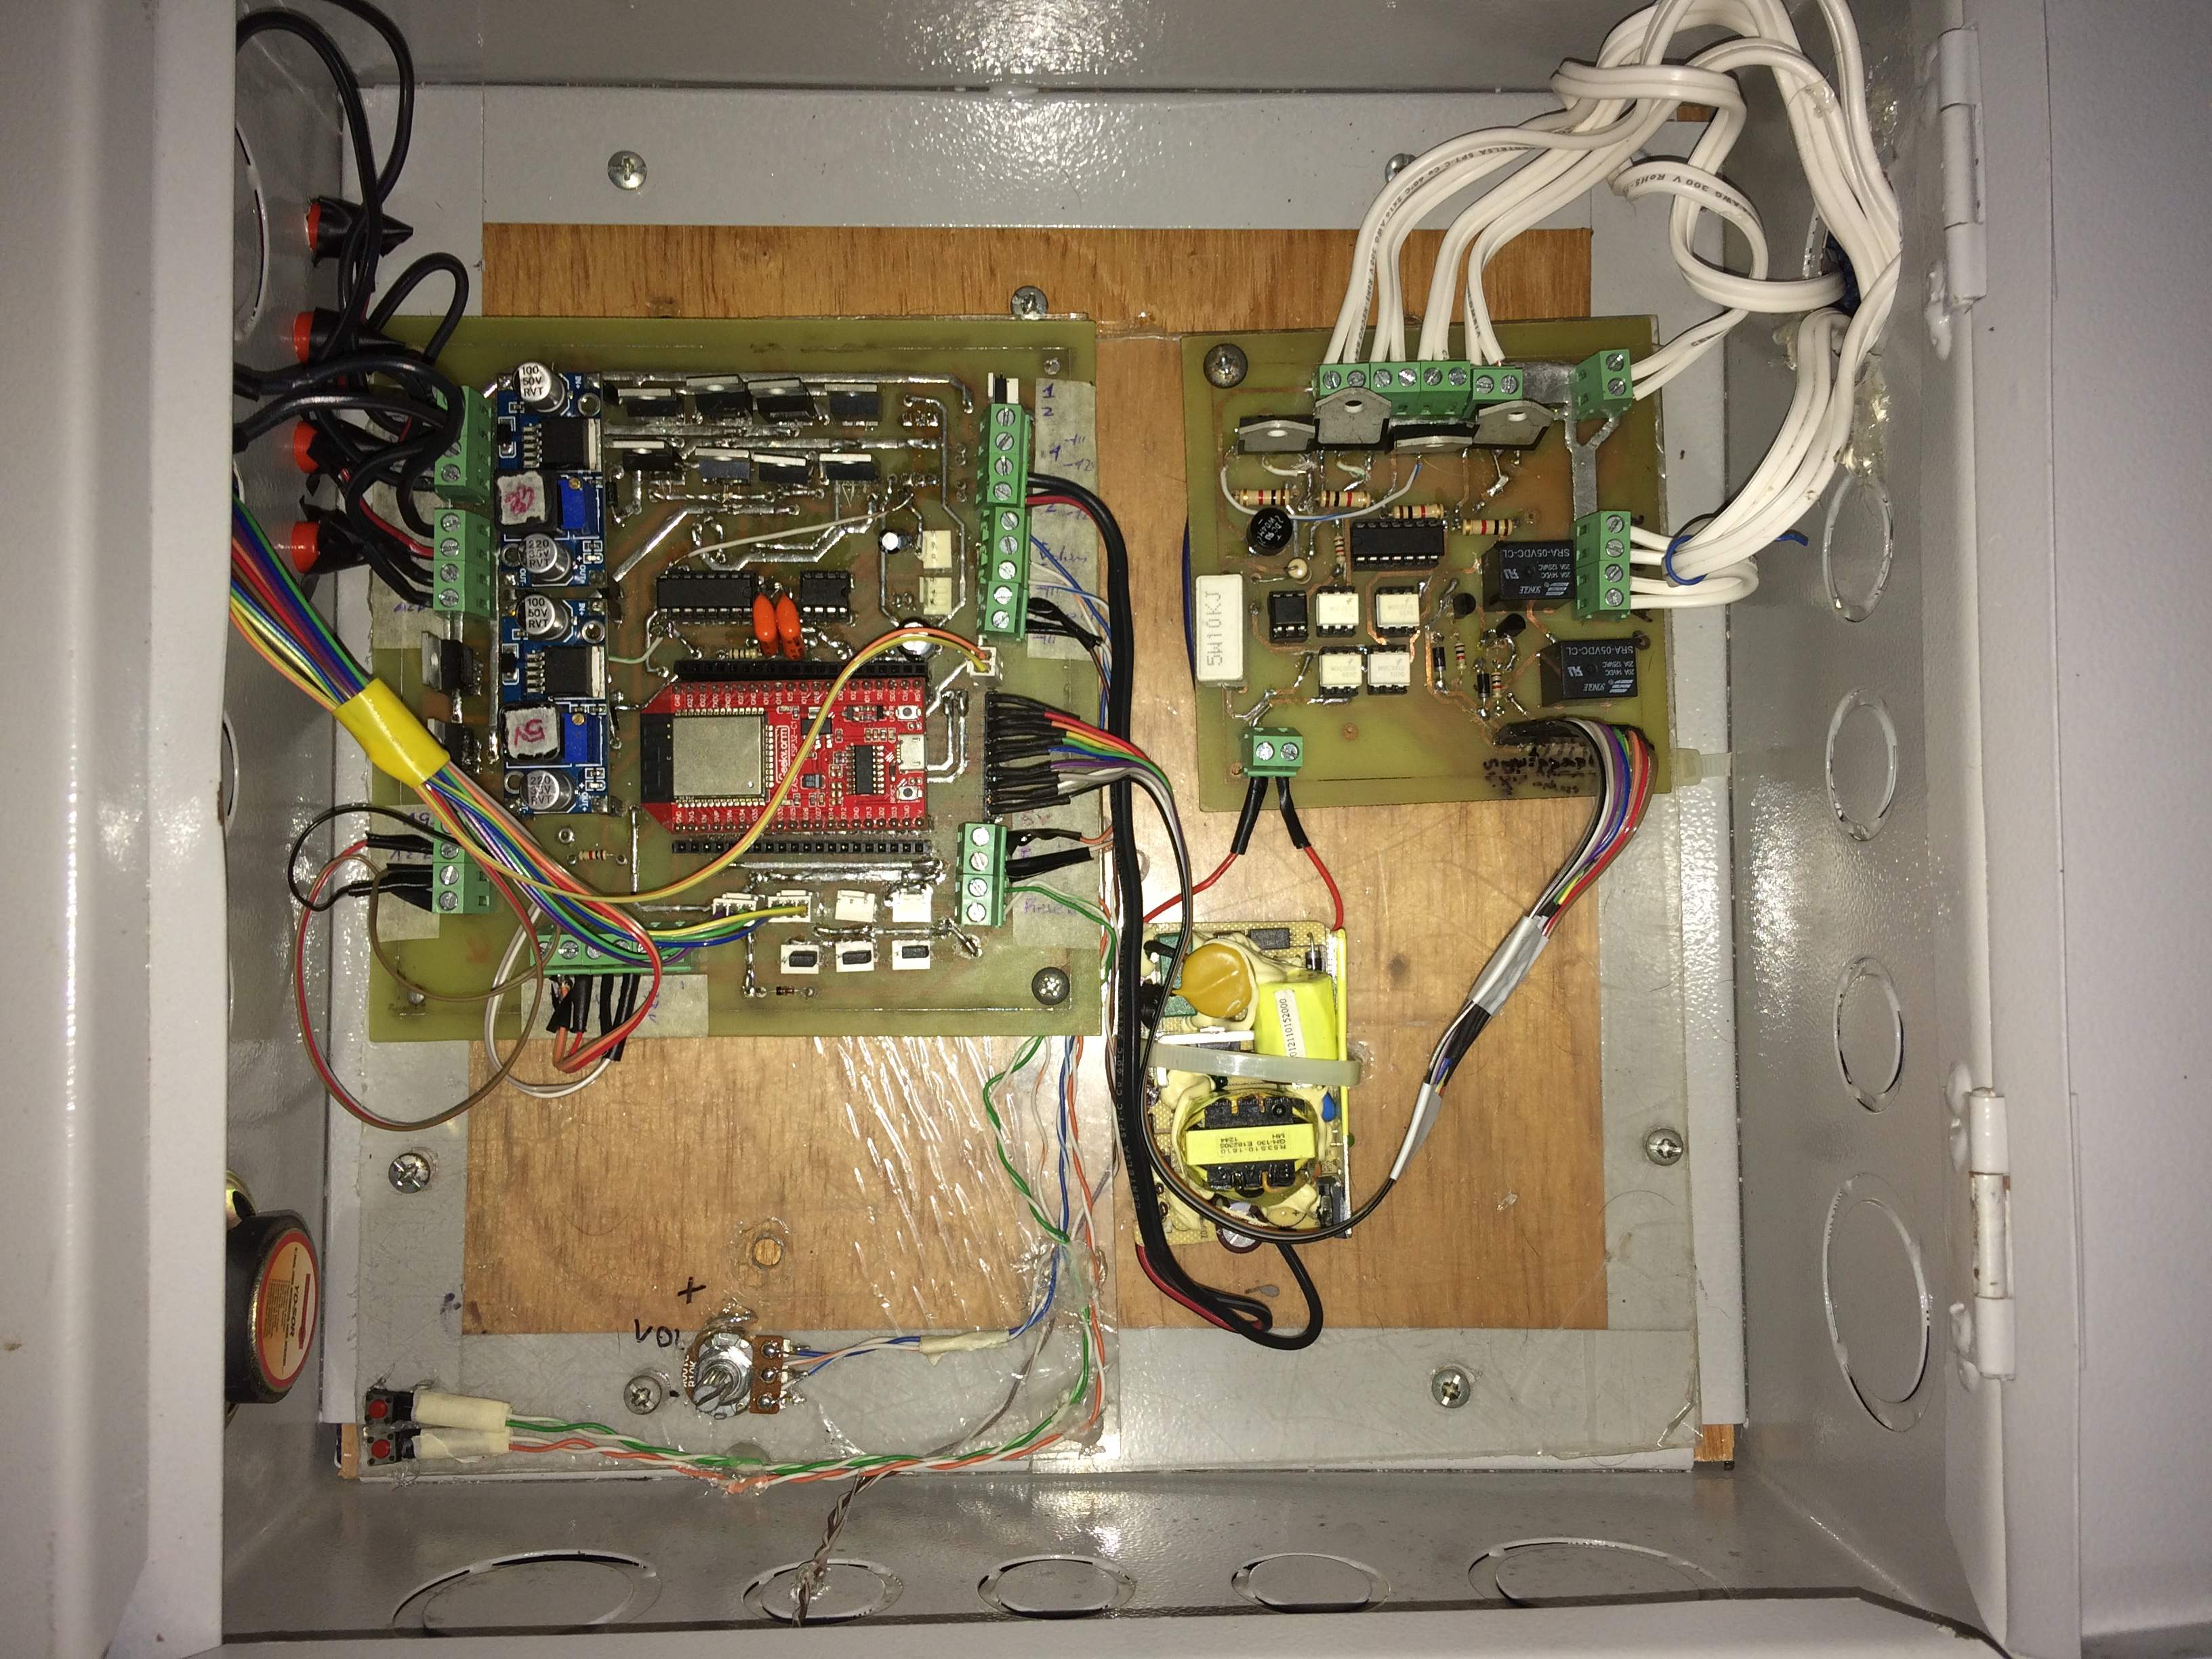
\includegraphics[width=0.6\linewidth]{Imagenes/Tarjeta}
\end{figure}

\begin{figure}[!t]
	\centering
	\caption{Descripción caja eléctrica tarjeta SmartHouse [Imagen Propia]}
	\label{fig:labels}
	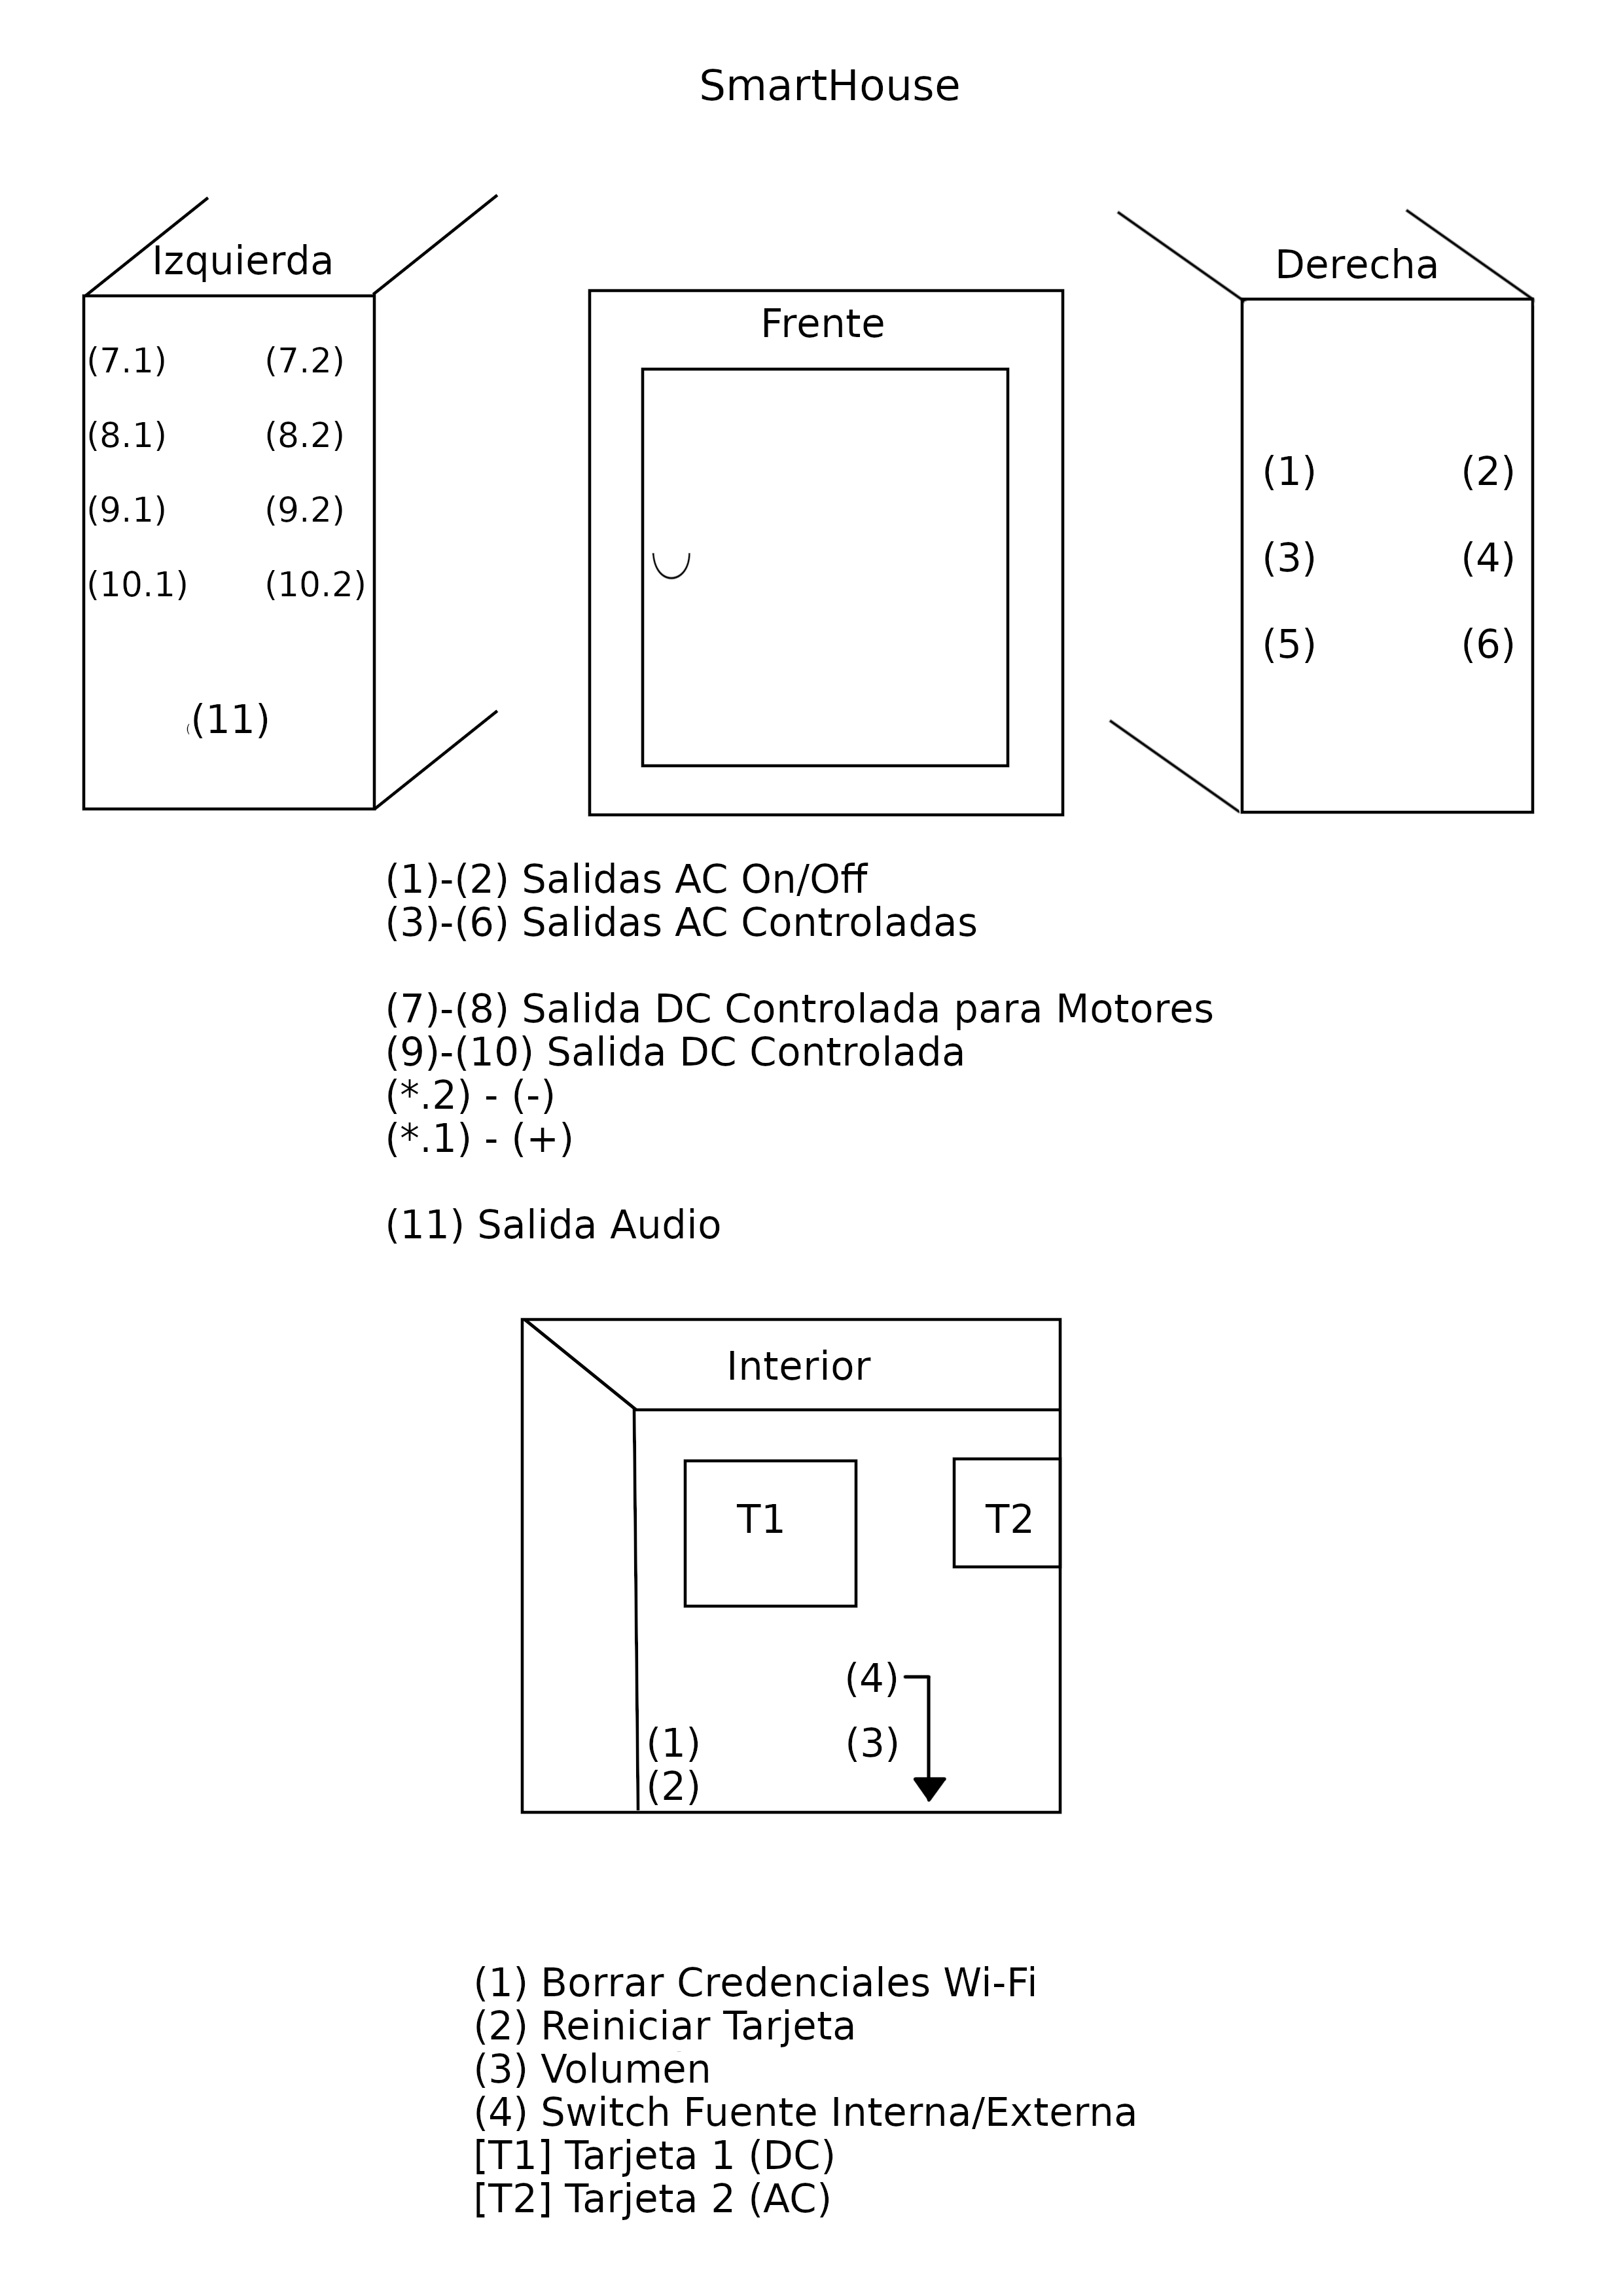
\includegraphics[width=0.7\linewidth]{Imagenes/labels}
\end{figure}

Conforme a lo mencionado anteriormente, el sistema se ha probado con cargas AC como bombillos LED entre 7W y 20W, de filamento de 100W, probando funcionalidades como el control de potencia AC por ángulo de fase, obteniendo los resultados esperados, según se observa en la figura \ref{fig:ACc}\textbf{(a)} donde la carga tiene el 100\% de la potencia y en la figura \ref{fig:ACc}\textbf{(b)} con el 20\% de esta. El voltaje de alimentación viene dado por la red eléctrica, la tarjeta simplemente conmuta el estado de la alimentación o controla la potencia entregada. \\

\begin{figure}[!t]
	\centering
	\caption{Control de potencia AC por ángulo de fase [Imagen Propia]}
	\label{fig:ACc}
	\subfigure[Potencia al 100\%]{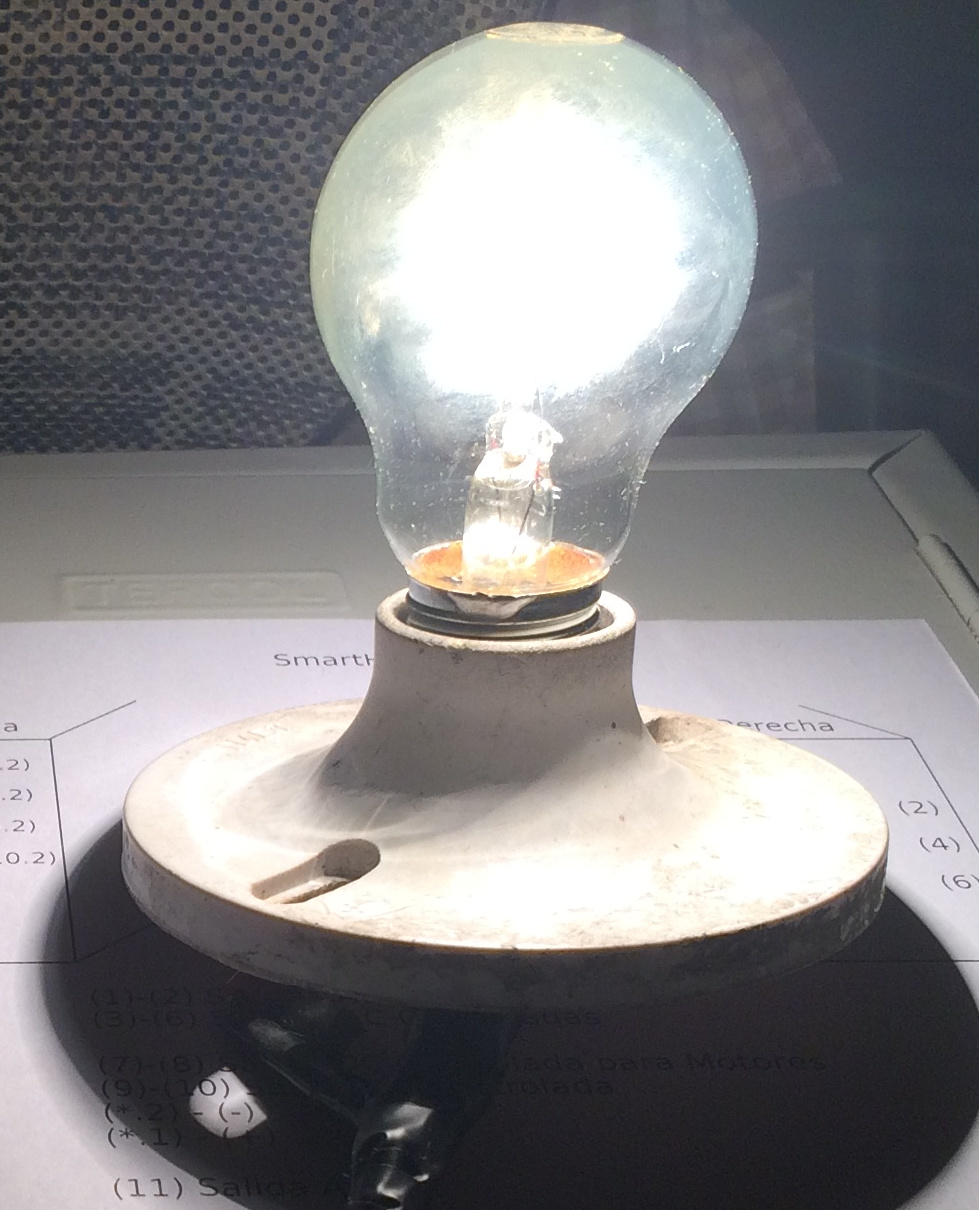
\includegraphics[width=0.45\linewidth]{Imagenes/AC1}}
	\subfigure[Potencia al 20\%]{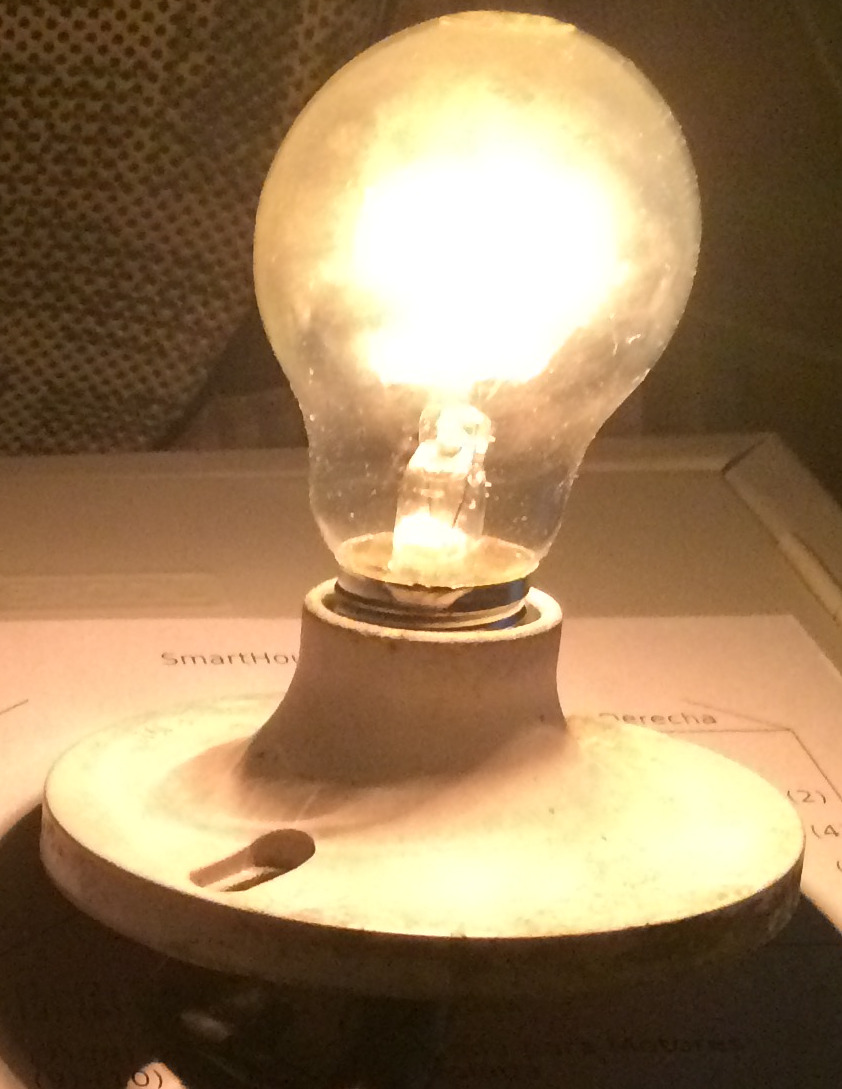
\includegraphics[width=0.43\linewidth]{Imagenes/AC0}}
\end{figure}

Para las salidas DC se realizan pruebas con un motor DC de 1W, además de una tira LED de 1W, la cual se le varia la energía entrega, como se observa en la figura \ref{fig:DCc}\textbf{(a)} la carga tiene el 100\% de la energía y en la figura \ref{fig:DCc}\textbf{(b)} solamente el 10\%. Estas cargas se alimentan con 12VDC directamente desde la fuente o convertidor AC-DC, los circuitos que se implementan simplemente conmutan el estado de encendido/apagado o por medio de PWM variar la energía entregada.\\

\begin{figure}[!t]
	\centering
	\caption{Control de Cargas DC [Imagen Propia]}
	\label{fig:DCc}
	\subfigure[Potencia al 100\%]{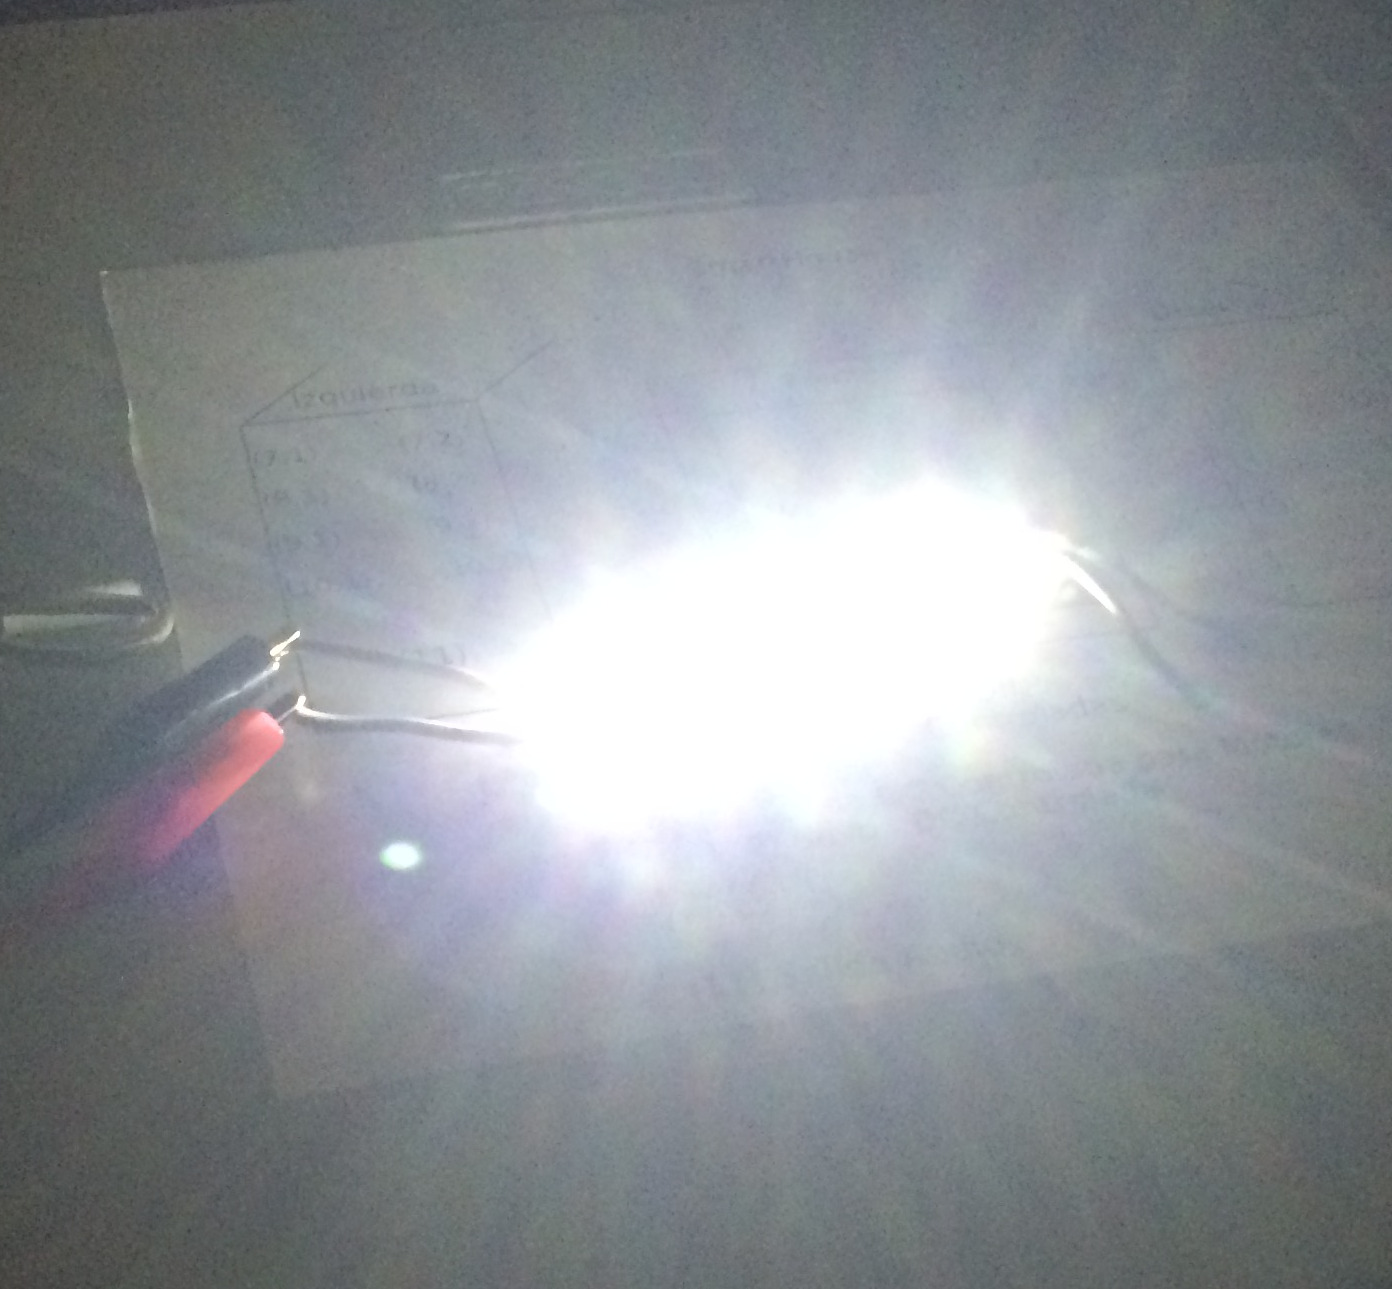
\includegraphics[width=0.45\linewidth]{Imagenes/DC1}}
	\subfigure[Potencial al 10\%]{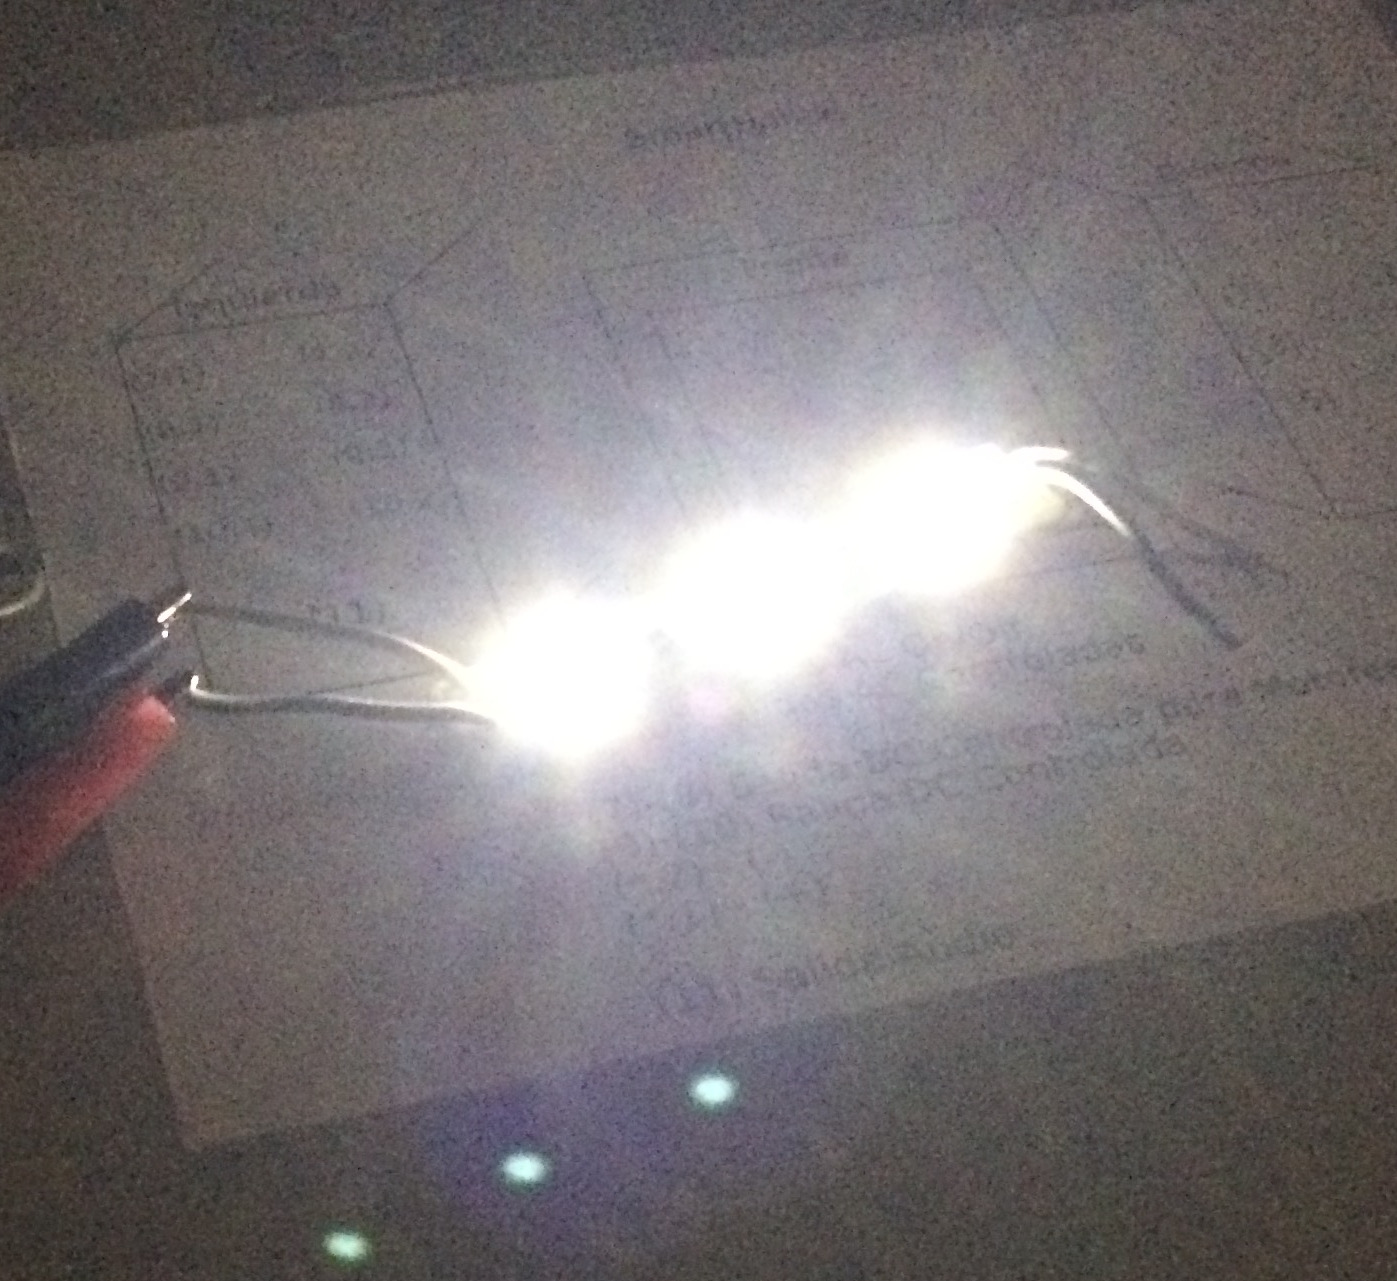
\includegraphics[width=0.455\linewidth]{Imagenes/DC0}}
\end{figure}

Se observa que el hardware quedo dividido en dos tarjetas, esto para facilitar la construcción y distribución de los diferentes elementos utilizados, si se usan componentes superficiales y se aumentan las capas de la tarjeta es posible reducir el tamaño y hasta integrarlas en una sola board. En la construcción de estas tarjetas se comprende diferentes funcionamientos en cuanto a los triac y los transistores mosfet, reforzando conocimientos que se habían adquirido.\\

\subsection{Prueba Beta Cerrada} 

Para la prueba beta se escoge un grupo de personas, las cuales interactúan directamente con la aplicación web y el prototipo de la tarjeta SmartHouse; en esta prueba se detallan diferentes ítems a evaluar, como el ingreso a la aplicación, visualización de los datos almacenados en esta y el control de los dispositivos; así, para evaluar estas características se califican de acuerdo con una escala tipo likert \cite{lik} de uno a cinco en la cual, cinco es la calificación máxima y uno la mínima.\\

La prueba se realiza a quince personas, entre los cuales algunos son estudiantes de ingería electrónica y personas ajenas a este tipo de escenarios, los resultados de la prueba se consignan en la tabla \ref{table:enc}, realizando el promedio de cada pregunta y presentando un resultado total.\\

\begin{table}
	\begin{center}
		\caption{Resultados por pregunta.}
		\label{table:enc}
		\begin{tabular}{|c|c|}
			\hline 
			\textbf{Número de la Pregunta} & \textbf{Promedio} \\ 
			\hline 
			1 & 4.5\\ 
			\hline 
			2 & 4.8\\ 
			\hline 
			3 & 4.5\\ 
			\hline 
			4 & 5.0\\ 
			\hline 
			5 & 4.9\\ 
			\hline 
			6 & 4.9\\ 
			\hline 
			7 & 4.3\\ 
			\hline 
			8 & 4.3\\ 
			\hline 
			9 & 4.8\\ 
			\hline 
			\textbf{Total} & \textbf{4.7}\\ 
			\hline 
		\end{tabular} 
	\end{center}
\end{table}

En resumen, el sistema recibe una calificación de 4.7, por lo tanto se puede decir que las funcionalidades requeridas están programadas de una manera adecuada y simple para que el usuario disponga de ellas, pero es posible mejorarlas con el objetivo de que sean mucho más intuitivas para el usuario y que no se le presenten dudas al momento de usarla. Conforme a las observaciones obtenidas durante la prueba se han modificado algunas partes del sistema, que no tienen un impacto significativo sobre los objetivos ni alcances propuestos en este trabajo.\\

Algunas características importantes resultantes de la prueba, recaen en la organización del hardware, de tal manera que sea más intuitiva la conexión y la manipulación de los botones, los cuales requieren un posicionamiento visualmente más cómodo dentro de la caja eléctrica en la que se encuentra el sistema. Por otra parte, el manual requiere modificaciones en la explicación de algunos procesos, ya que a pesar de que este permite el manejo correcto del sistema, requiere mayor detalle en procedimientos que requieren conocer aspectos como el manejo de un dispositivo inteligente o claridad adicional al usar el dispositivo por primera vez.\\

Además de esto, es importante resaltar que las interacciones de los usuarios a través de la aplicación web se realizan de manera fácil y entendible, pues los aspectos relacionados con esta y su navegación, mantienen el promedio más alto de la prueba, dejando claro que este aspecto del sistema tuvo gran éxito en cuanto a los usuarios se refiere.\\

\section{Conclusiones}

\begin{itemize}
	\item El sistema compuesto de Firmware, Hardware y Software descrito en este documento es una solución IoT funcional, ya que este cuenta con la capacidad de monitorear y controlar un entorno de aplicación por medio de internet, el cual es en este caso una habitación de Smart House, siendo esta la representación de uno de los infinitos escenarios posibles a los cuales puede ser conectado el sistema, puesto que está diseñado con el fin de abarcar un amplio número de tareas, además de que acepta múltiples tipos de dispositivos de medida; combinando estos aspectos con una PaaS que permite la interacción humano-maquina, de tal manera que cumple con las características principales para una solución IoT.\\
	
	\item El hardware implementado para la solución IoT, funciona en conjunto con el firmware que enlaza su parte física con el software presente en la nube; este fue diseñado en dos etapas con un circuito para cada una, las cuales son la etapa de potencia AC y la etapa DC. Esta organización del sistema no solo permite una clasificación en cuanto a su funcionamiento, sino que también evita que los altos voltajes de la etapa AC causen algún tipo de interferencia de manera directa con la etapa DC. Cada etapa del hardware cuenta con una alimentación que garantiza los niveles correctos para la alimentación de los sensores y cargas, además de una apropiada lectura de cada dispositivo de medida y una adecuada manipulación del entorno.\\
	
	\item La aplicación web presentada en este documento, permite la interacción del usuario con los diferentes dispositivos que se encuentran conectados al hardware. Esta característica del sistema se encarga de la gestión de la información recolectada por el hardware junto con las órdenes administradas por el mismo, ya sea por visualización o manipulación del entorno de instalación, es decir, para su monitoreo o control, ya que se tiene acceso desde cualquier lugar con conexión a internet; de este modo la aplicación cumple con los diferentes alcances y puede seguir siendo ampliada a fin de adicionar funcionalidades al sistema. Con la implementación de este programa se han adquirido varios conocimientos sobre aplicaciones web y los lenguajes de programación que requieren, tales como PHP, JavaScript, entre otros.\\
	
	\item Realizar pruebas tales como la prueba Beta cerrada, represento una importante herramienta para la evaluación de características importantes del sistema con la participación de los usuarios finales, tales como el encendido y manipulación del entorno (hardware) junto con sus conexiones, así como también la navegación e interacción con la aplicación web (software). Debido a que el resultado de la prueba fue 4.7/5.0 demuestra que aún quedan algunos pequeños aspectos por enriquecer, pero también indica que cumple con la funcionalidad propuesta, con el objetivo de mejorar se debe mantener un estrecho contacto con el cliente recibiendo constantes opiniones.\\
	
	\item La tarjeta de prototipado ESP32 como unidad central de procesamiento dentro del desarrollo del hardware, representa una opción viable en la puesta en funcionamiento de un sistema IoT, no solo por su bajo costo sino también por sus características y funcionalidades, las cuales están diseñadas para este tipo de aplicaciones, permitiendo que el diseño y la implementación del sistema sea escalable, asimismo porque cuenta con un gran número de pines y diversas opciones para aumentar su capacidad.\\
	
	\item El uso del framework ESP-IDF, que se compone de un sistema operativo en tiempo real freeRTOS, es muy útil para realizar las diferentes funciones del sistema que comunica hardware con software, además de que permite ejecutar las diversas tareas y gestionar bien los recursos presentes en el chip ESP32, por lo tanto es posible agregar una amplia gama de características adicionales a la funcionalidad del sistema, gracias a que esta en constante expansión agregando nuevas opciones y diversos controladores para el ESP32.\\
	
\end{itemize}
%\section{Trabajos Futuros}

Como trabajo futuro en cuanto al hardware se propone integrar todo el sistema en una sola board, migrando la mayoría de componentes de montaje through hole a superficial (SMD) y también realizar un diseño con más capas, por ejemplo de cuatro capas, para reducir el tamaño de esta e incorporar todas las funcionalidades en una sola, además de añadir mas características a este, como el manejo de otros dispositivos por medio de infrarrojo, poder actualizar su firmware remotamente y funciones de ahorro de energía.\\

En el software es conveniente agregar funcionalidades de acuerdo con los otros roles presentes en este, por ejemplo para el rol usuario administrador de casa crear reglas de control parental y de seguridad con el fin de ampliar la administración sobre sus propios dispositivos.\\

En la parte de realización de la prueba del sistema se pueden realizar otros tipos como alfa, de aceptación, entre otras más que existen para probar los diferentes software diseñados, además ampliar la muestra en la que se aplican estas pruebas.\\

Para mejorar la solución IoT es posible crear servidores espejo localmente en la tarjeta incluyéndolo en el firmware y realizando copias de la información constantemente. Sus funcionalidades son en caso de mantenimiento de la aplicación principal o de cualquier problema relativo a la conexión a Internet, esta daría soporte local hasta que entre de nuevo en funcionamiento la que se encuentra en la nube.\\

%\section{Introduccion}
% The very first letter is a 2 line initial drop letter followed
% by the rest of the first word in caps.
% 
% form to use if the first word consists of a single letter:
% \IEEEPARstart{A}{demo} file is ....
% 
% form to use if you need the single drop letter followed by
% normal text (unknown if ever used by the IEEE):
% \IEEEPARstart{A}{}demo file is ....
% 
% Some journals put the first two words in caps:
% \IEEEPARstart{T}{his demo} file is ....
% 
% Here we have the typical use of a "T" for an initial drop letter
% and "HIS" in caps to complete the first word.
%\IEEEPARstart{T}{his} demo file is intended to serve as a ``starter file''
%for IEEE journal papers produced under \LaTeX\ using
%IEEEtran.cls version 1.8b and later.
%% You must have at least 2 lines in the paragraph with the drop letter
%% (should never be an issue)
%I wish you the best of success.
%
%\hfill mds
% 
%\hfill August 26, 2015

%\subsection{Subsection Heading Here}
%Subsection text here.

% needed in second column of first page if using \IEEEpubid
%\IEEEpubidadjcol

%\subsubsection{Subsubsection Heading Here}
%Subsubsection text here.


% An example of a floating figure using the graphicx package.
% Note that \label must occur AFTER (or within) \caption.
% For figures, \caption should occur after the \includegraphics.
% Note that IEEEtran v1.7 and later has special internal code that
% is designed to preserve the operation of \label within \caption
% even when the captionsoff option is in effect. However, because
% of issues like this, it may be the safest practice to put all your
% \label just after \caption rather than within \caption{}.
%
% Reminder: the "draftcls" or "draftclsnofoot", not "draft", class
% option should be used if it is desired that the figures are to be
% displayed while in draft mode.
%
%\begin{figure}[!t]
%\centering
%\includegraphics[width=2.5in]{myfigure}
% where an .eps filename suffix will be assumed under latex, 
% and a .pdf suffix will be assumed for pdflatex; or what has been declared
% via \DeclareGraphicsExtensions.
%\caption{Simulation results for the network.}
%\label{fig_sim}
%\end{figure}

% Note that the IEEE typically puts floats only at the top, even when this
% results in a large percentage of a column being occupied by floats.


% An example of a double column floating figure using two subfigures.
% (The subfig.sty package must be loaded for this to work.)
% The subfigure \label commands are set within each subfloat command,
% and the \label for the overall figure must come after \caption.
% \hfil is used as a separator to get equal spacing.
% Watch out that the combined width of all the subfigures on a 
% line do not exceed the text width or a line break will occur.
%
%\begin{figure*}[!t]
%\centering
%\subfloat[Case I]{\includegraphics[width=2.5in]{box}%
%\label{fig_first_case}}
%\hfil
%\subfloat[Case II]{\includegraphics[width=2.5in]{box}%
%\label{fig_second_case}}
%\caption{Simulation results for the network.}
%\label{fig_sim}
%\end{figure*}
%
% Note that often IEEE papers with subfigures do not employ subfigure
% captions (using the optional argument to \subfloat[]), but instead will
% reference/describe all of them (a), (b), etc., within the main caption.
% Be aware that for subfig.sty to generate the (a), (b), etc., subfigure
% labels, the optional argument to \subfloat must be present. If a
% subcaption is not desired, just leave its contents blank,
% e.g., \subfloat[].


% An example of a floating table. Note that, for IEEE style tables, the
% \caption command should come BEFORE the table and, given that table
% captions serve much like titles, are usually capitalized except for words
% such as a, an, and, as, at, but, by, for, in, nor, of, on, or, the, to
% and up, which are usually not capitalized unless they are the first or
% last word of the caption. Table text will default to \footnotesize as
% the IEEE normally uses this smaller font for tables.
% The \label must come after \caption as always.
%
%\begin{table}[!t]
%% increase table row spacing, adjust to taste
%\renewcommand{\arraystretch}{1.3}
% if using array.sty, it might be a good idea to tweak the value of
% \extrarowheight as needed to properly center the text within the cells
%\caption{An Example of a Table}
%\label{table_example}
%\centering
%% Some packages, such as MDW tools, offer better commands for making tables
%% than the plain LaTeX2e tabular which is used here.
%\begin{tabular}{|c||c|}
%\hline
%One & Two\\
%\hline
%Three & Four\\
%\hline
%\end{tabular}
%\end{table}


% Note that the IEEE does not put floats in the very first column
% - or typically anywhere on the first page for that matter. Also,
% in-text middle ("here") positioning is typically not used, but it
% is allowed and encouraged for Computer Society conferences (but
% not Computer Society journals). Most IEEE journals/conferences use
% top floats exclusively. 
% Note that, LaTeX2e, unlike IEEE journals/conferences, places
% footnotes above bottom floats. This can be corrected via the
% \fnbelowfloat command of the stfloats package.




%\section{Conclusion}
%The conclusion goes here.

% if have a single appendix:
%\appendix[Proof of the Zonklar Equations]
% or
%\appendix  % for no appendix heading
% do not use \section anymore after \appendix, only \section*
% is possibly needed

% use appendices with more than one appendix
% then use \section to start each appendix
% you must declare a \section before using any
% \subsection or using \label (\appendices by itself
% starts a section numbered zero.)
%


%\appendices
%\section{Proof of the First Zonklar Equation}
%Appendix one text goes here.
%
%% you can choose not to have a title for an appendix
%% if you want by leaving the argument blank
%\section{}
%Appendix two text goes here.


% use section* for acknowledgment
%\section*{Acknowledgment}
%
%
%The authors would like to thank...


% Can use something like this to put references on a page
% by themselves when using endfloat and the captionsoff option.
%\ifCLASSOPTIONcaptionsoff
%  \newpage
%\fi



% trigger a \newpage just before the given reference
% number - used to balance the columns on the last page
% adjust value as needed - may need to be readjusted if
% the document is modified later
%\IEEEtriggeratref{8}
% The "triggered" command can be changed if desired:
%\IEEEtriggercmd{\enlargethispage{-5in}}

% references section

% can use a bibliography generated by BibTeX as a .bbl file
% BibTeX documentation can be easily obtained at:
% http://mirror.ctan.org/biblio/bibtex/contrib/doc/
% The IEEEtran BibTeX style support page is at:
% http://www.michaelshell.org/tex/ieeetran/bibtex/
%\bibliographystyle{IEEEtran}
% argument is your BibTeX string definitions and bibliography database(s)
%\bibliography{IEEEabrv,../bib/paper}
%
% <OR> manually copy in the resultant .bbl file
% set second argument of \begin to the number of references
% (used to reserve space for the reference number labels box)
\begin{thebibliography}{1}

%\bibitem{IEEEhowto:kopka}
%H.~Kopka and P.~W. Daly, \emph{A Guide to \LaTeX}, 3rd~ed.\hskip %1em plus
  %0.5em minus 0.4em\relax Harlow, England: Addison-Wesley, 1999.
  
  \bibitem{Behan2013}
  Miroslav Behan and Ondrej Krejcar, \emph{Vision of Smart Home Point Solution as Sustainable Intelligent House Concept}, 2013.
  
  \bibitem{Cheuque2015}
  	César Cheuque and Felipe Baeza and Gastón Márquez and Juan Calderón, \emph{Towards to responsive Web Services for Smart Home LED control with Raspberry Pi. A first approach}, 2015.
  	
	\bibitem{Kusriyanto2015}
  	Medilla Kusriyanto and Beny Setiawan, \emph{Android Smart Home System Based on ATmega16}, 2015.
  	
  	\bibitem{Kaneko2017}
  	Masayuki Kaneko and Kazuki Arima and Takashi Murakami and Masao Isshiki and Hiroshi Sugimura, \emph{Design and Implementation of Interactive Control System for Smart Houses}, 2017.
  	
  	\bibitem{Asthon2009}
  	Kevin Ashton, \emph{That 'Internet of Things' Thing}, 2009.
  	
  	\bibitem{JSON}
  	JSON.org, \emph{Introducción a JSON}. 
  	
  	\bibitem{EW32}
  	Espressif Systems, \emph{ESP-WROOM-32 Datasheet}, 2018.
  	
  	\bibitem{ESPIMG}
  	Electrodragon, \emph{ESP-WROOM-32}.
  
  	\bibitem{CEKIT}
  	CEKIT, \emph{Curso práctico de Electrónica Inductrial y Automatización}, 2001.
  	
  	\bibitem{PWM}
  	Enrique Gómez, \emph{Qué es PWM y para qué sirve}, 2017.
  	
  	\bibitem{ES}
  	Espressif Systems, \emph{ESP-IDF Programming Guide}.
  	
  	\bibitem{DC0}
  	platea pntic, \emph{DISPARADORES DE SCHMITT}.
  	
  	\bibitem{LM386}
  	Texas Instrument, \emph{LM386 Low Voltage Audio Power Amplifier}.
  	
  	\bibitem{MVC1}
  	Juan Pavón Mestras, \emph{Estructura de las Aplicaciones Orientadas a Objetos
  		El patrón Modelo-Vista-Controlador (MVC)}, 2009.
  	
  	\bibitem{Eloq}
  	Richos, \emph{Libro Laravel 5 Conceptos básicos y ejemplos}, 2016.  	
  	
  	\bibitem{PB}
  	Universidad de Sevilla, \emph{Técnicas de evluación	Dinámica}.
  	
  	\bibitem{lik}
  	BPO Centro de Comercio, \emph{LA ESCALA DE LIKERT: QUÉ ES Y CÓMO UTILIZARLA}, 2016.

\end{thebibliography}

% biography section
% 
% If you have an EPS/PDF photo (graphicx package needed) extra braces are
% needed around the contents of the optional argument to biography to prevent
% the LaTeX parser from getting confused when it sees the complicated
% \includegraphics command within an optional argument. (You could create
% your own custom macro containing the \includegraphics command to make things
% simpler here.)
%\begin{IEEEbiography}[{\includegraphics[width=1in,height=1.25in,clip,keepaspectratio]{mshell}}]{Michael Shell}
% or if you just want to reserve a space for a photo:

%\begin{IEEEbiography}{Michael Shell}
%Biography text here.
%\end{IEEEbiography}

% if you will not have a photo at all:
%\begin{IEEEbiographynophoto}{John Doe}
%Biography text here.
%\end{IEEEbiographynophoto}

% insert where needed to balance the two columns on the last page with
% biographies
%\newpage

%\begin{IEEEbiographynophoto}{Jane Doe}
%Biography text here.
%\end{IEEEbiographynophoto}

% You can push biographies down or up by placing
% a \vfill before or after them. The appropriate
% use of \vfill depends on what kind of text is
% on the last page and whether or not the columns
% are being equalized.

%\vfill

% Can be used to pull up biographies so that the bottom of the last one
% is flush with the other column.
%\enlargethispage{-5in}



% that's all folks
\end{document}


